\documentclass[3p,times]{elsarticle}

%% The `ecrc' package must be called to make the CRC functionality available
\usepackage{ecrc}
%% The ecrc package defines commands needed for running heads and logos.
%% For running heads, you can set the journal name, the volume, the starting page and the authors

%% set the volume if you know. Otherwise `00'
\volume{00}

%% set the starting page if not 1
\firstpage{1}

%% Give the name of the journal
\journalname{}

%% Give the author list to appear in the running head
%% Example \runauth{C.V. Radhakrishnan et al.}
\runauth{}

%% The choice of journal logo is determined by the \jid and \jnltitlelogo commands.
%% A user-supplied logo with the name <\jid>logo.pdf will be inserted if present.
%% e.g. if \jid{yspmi} the system will look for a file yspmilogo.pdf
%% Otherwise the content of \jnltitlelogo will be set between horizontal lines as a default logo

%% Give the abbreviation of the Journal.
\jid{procs}

%% Give a short journal name for the dummy logo (if needed)
\jnltitlelogo{}

%% Hereafter the template follows `elsarticle'.
%% For more details see the existing template files elsarticle-template-harv.tex and elsarticle-template-num.tex.

%% Elsevier CRC generally uses a numbered reference style
%% For this, the conventions of elsarticle-template-num.tex should be followed (included below)
%% If using BibTeX, use the style file elsarticle-num.bst

%% End of ecrc-specific commands
%%%%%%%%%%%%%%%%%%%%%%%%%%%%%%%%%%%%%%%%%%%%%%%%%%%%%%%%%%%%%%%%%%%%%%%%%%

%% The amssymb package provides various useful mathematical symbols
\usepackage{amssymb}
%% The amsthm package provides extended theorem environments
\usepackage{amsthm}
\usepackage{amsmath}
\usepackage{algorithm2e}
\usepackage{graphicx}
\usepackage{subcaption}
\usepackage{hyperref}

\usepackage{xcolor}
\usepackage[version=4]{mhchem}
\newcommand{\N}{\mathbb{N}}
\newcommand{\R}{\mathbb{R}}
\newcommand{\I}{\mathcal{I}}
\newcommand{\diag}{\textbf{diag}}
\newtheorem{defn}{Definition}
\newtheorem{hypo}{H}
\newtheorem{lemma}{Lemma}
\newtheorem{theo}{Theorem}
%% The lineno packages adds line numbers. Start line numbering with
%% \begin{linenumbers}, end it with \end{linenumbers}. Or switch it on
%% for the whole article with \linenumbers after \end{frontmatter}.
%% \usepackage{lineno}

%% natbib.sty is loaded by default. However, natbib options can be
%% provided with \biboptions{...} command. Following options are
%% valid:

%%   round  -  round parentheses are used (default)
%%   square -  square brackets are used   [option]
%%   curly  -  curly braces are used      {option}
%%   angle  -  angle brackets are used    <option>
%%   semicolon  -  multiple citations separated by semi-colon
%%   colon  - same as semicolon, an earlier confusion
%%   comma  -  separated by comma
%%   numbers-  selects numerical citations
%%   super  -  numerical citations as superscripts
%%   sort   -  sorts multiple citations according to order in ref. list
%%   sort&compress   -  like sort, but also compresses numerical citations
%%   compress - compresses without sorting
%%
%% \biboptions{comma,round}

% \biboptions{}

% if you have landscape tables
\usepackage[figuresright]{rotating}

\graphicspath{{Images/}}
% put your own definitions here:
%   \newcommand{\cZ}{\cal{Z}}
%   \newtheorem{def}{Definition}[section]
%   ...

% add words to TeX's hyphenation exception list
%\hyphenation{author another created financial paper re-commend-ed Post-Script}

% declarations for front matter

\begin{document}

\begin{frontmatter}

%% Title, authors and addresses

%% use the tnoteref command within \title for footnotes;
%% use the tnotetext command for the associated footnote;
%% use the fnref command within \author or \address for footnotes;
%% use the fntext command for the associated footnote;
%% use the corref command within \author for corresponding author footnotes;
%% use the cortext command for the associated footnote;
%% use the ead command for the email address,
%% and the form \ead[url] for the home page:
%%
%% \title{Title\tnoteref{label1}}
%% \tnotetext[label1]{}
%% \author{Name\corref{cor1}\fnref{label2}}
%% \ead{email address}
%% \ead[url]{home page}
%% \fntext[label2]{}
%% \cortext[cor1]{}
%% \address{Address\fnref{label3}}
%% \fntext[label3]{}

\dochead{}
%% Use \dochead if there is an article header, e.g. \dochead{Short communication}

\title{Microbial interactions as drivers of a nitrifying ecosystem in a chemostat}
%% \title{Correcting/Improving chemostat models from microbial interactions}
%% Including microbial ecology in a chemostat model: tracking microbial interactions
%% 
%% Extending a chemostat model 
%% use optional labels to link authors explicitly to addresses:
%% \author[label1,label2]{<author name>}
%% \address[label1]{<address>}
%% \address[label2]{<address>}

\author{Pablo Ugalde-Salas, Jérôme Harmand, Elie Desmond Le-Quéméner, Héctor Ramirez}

\address{}

\begin{abstract}
	This article deals with the inclusion of microbial ecology measurements in bioprocess modelling. The first part presents the mathematical analysis of a model that may be framed within the class of Lotka-Volterra models fitted to experimental data in a chemostat setting. The limitations and the insights of such an approach are discussed. The main novelty of this work lies in the second part, where the use of an optimal tracking technique (developed within the framework of control theory) for the integration of genetic sequencing in chemostat models is presented. The method revisits the data used in the aforementioned chemostat setting. 
\end{abstract}

\end{frontmatter}

\section{Introduction}


Microbial communities and their interactions play a central role in the understanding of microbial ecosystems \cite{West2007}, and a current challenge is integrating genetic sequencing data in a deterministic modelling framework \cite{Widder2016,WADE201664}. A thorough review in current methodologies in the deterministic modelling approaches of microbial community dynamics is presented by Song \textit{et al.} \cite{Song2014}. Using their terminology this articles deals with population-based approaches where species are taken as the interacting units.

The classical ecological concept of species and niche in the microbial world is an elusive one: In the macro world one can clearly identify one species of another for reproductive reasons and their ability to give birth to offspring. In the case of bacteria and archea, reproduction goes simply by binary fission and exchange of some functional genes (the ability to synthesize or metabolize substances) can be acquired in evolutionary scale through lateral gene transfer \cite{Boucher2003}. Therefore as an ecological problem is hard to precise the 'niche' of 'species'.

These obstacles can be circumvented by considering the microbiologist concept of operative taxonomic unit (OTU) based on the clustering of organisms sharing similar sequences of 16S rDNA marker gene. There is a core genome in Bacteria, which is in turn related to the main metabolism of Bacteria, and thus their 'function' within a given ecosystem. The function of an OTU, from an engineering perspective, is given by which substances are transformed and at which growth rates and substrate to biomass conversion yields \cite{Muyzer1993}.

In the past years considerable efforts have been made to measure the bacterial community composition. Tests such as fluorescence in situ hybridization, polymerase chain reaction (PCR) dependent techniques, and PCR independent techniques for the analysis of DNA, RNA, proteins, and metabolites have become a standard tool for studying  microbial diversity\cite{FERRERA2016790}. 

The contribution of this article is a new method to integrate the microbial community measurements in chemostat models, based on any sequencing or fingerprinting technique that can quantify the species abundances over time. This is a first step towards developing predictive models of a reactor's outcome based on the microbial community structure.

As a departing point the work of Dumont et al.\cite{Dumont2016} is reinspected in section 2. They model a chemostat experiment where nitrification takes place by considering a generalized Lotka-Volterra (gLV) model \cite{Hernandez-Bermejo1997} coupled with a substrate limited growth expression. Section 3 inspects through a mathematical analysis their model. Some interesting outputs of this analysis are that the number of possible equilibrium points grows exponentially with the number of species,  coexistence can be achieved within the same functional group, and bi-stability may arise.  

In section 4 the concept of interaction function is developed such that it generalizes the gLV model. For the identification of the interaction function a method of optimal control theory was adapted: The growth rate of each species is modulated by a constrained regular control of the system, thus the growth rate of each OTU is corrected in order to fit the experimental data. The regular control is composed of a feedback part on the species state variable, and a feed forward part, or tracking, on the measurement of abundances of each species; the method involves solving state-dependent Ricatti equations\cite{Cimen2008}. 

In section 5 the methodology from section 4 is applied to the data from the experiments performed by Dumont \textit{et al}\cite{Dumont2009} and not just to the most abundant species as it was the case of the model analysed in section 3 \cite{Dumont2016}. The method shows that by following the community dynamics one can propose a growth rate that reconstructs the substrates dynamics. The article ends with a discussion on the scope of applicability of the method and perspectives. 

\section{Model Definition}

Notations used throughout the article:
\begin{enumerate}
	\item $n$: the number of OTU considered.
	\item $n_i, \, i \in \{1,2\}$: the number of OTU in functional group $G_i$.
	\item Let $m$ be an interger then $[m]:=\{1,\dots,n \}$. 
	\item $x_i$ :  is the concentration of OTU $i$ measured in $[g/l]$. $i \in [n]$. 
	\item $x$: vector $(x_1,\dots,x_n)^\top$.
	\item $s_1$ : concentration of substrate 1 in $[g/l]$.
	\item $s_2$ : concentration of substrate 2 in $[g/l]$. 
	\item $s_3$ : concentration of substrate 3 in $[g/l]$.
	\item $s$:  vector $(s_1,s_2,s_3)$. Refered to as metabolites, or chemical species.
	\item $\I_i(t,x)$ : Interaction function of OTU $i \in \{1,\dots,n\}$.
	\item $\mu_i(s,x)$ : growth function of OTU $i \in \{1,\dots,n\}$.
	\item $\mu = (\mu_1(s,x), \dots, \mu_n(s,x))$ vector containing the growth function of every OTU.
	\item $D$: dilution rate of the continuous reactor in $[1/day]$. 
	\item $y_i$: yield of moles of biomass formed per mole of substrate consumed of OTU $i$.
	\item $y$: vector $y_1,\dots,y_n$.
	\item $k_i$: yield of  moles of substrate consumed per mole of biomass formed of OTU $i$ . The inverse of the biomass yield $k_i = \dfrac{1}{y_i}$.
	\item $k$: vector $k_1,\dots,k_n$.
	\item For integers $m_1$ and $m_2$ and $a \in \R$, $a_{m_1 \times m_2}$ represents a matrix of $m_1$ rows and $m_2$ columns with $a$ in every entry. 
	\item Let $m$ be an integer then $I_m$ is the identity matrix of size $m$.
	\item Let $S$ be a finite set with $m \in \N$ elements. Then $\vert S \vert := m$. 
\end{enumerate}

\subsection{Stoichiometric Equations}
A cascade (bio)reaction process is considered. Suppose $n$ different OTU are present in the chemostat. The cascade reaction refers to the situation where a group of microorganisms ($G_1 \subset [n] $) consumes a substrate $s_1$ and produces $s_2$ and biomass, while another group of microorganisms ($G_2\subset [n]$) consumes $s_2$ and produces $s_3$ and biomass. $G_1$ and $G_2$ are called functional groups. The number of organisms in each functional will be denoted $n_1$ and $n_2$ respectively, that is $\vert G_1 \vert = n_1$ and $\vert G_2 \vert = n_2$ . This work treats the case when $G_1$ and $G_2$ are disjoint sets:

\begin{hypo}  Sets $G_1$ and $G_2$ satisfy: $G_1 \cap G_2 = \emptyset$ and $G_1 \cup G_2 = [n]$. 
\end{hypo}

The situation is described as simplified reactions \eqref{Reaction1} and \eqref{Reaction2}. The reactions are simplified in the sense that they do not attempt to represent a balanced chemical reaction, rather it represents the direction of the bioprocess and the proportions of different consumed and formed compounds of interest. 

The terms $y_i$ are known as yields, they represent the number of grams of biomass produced per gram of substrate consumed for OTU $i$. In this work the unit grams of dry biomass per gram of substrate is used for yields. Furthermore, for each $ i \in [n]$, OTU $i$ is characterized by its process rate (also known as growth function) $\mu_i(s,x)$. Notice that for being as generic as possible, the growth rate may be a function of the whole state in order to model the influence of all OTU on the growth rates of others.
\begin{align}
\label{Reaction1} \tag{R G1} 	s_1 \stackrel{\mu_i(s,x)}{\longrightarrow} s_2 + y_ix_i \quad \forall i \in G_1 \\
\label{Reaction2} \tag{R G2} s_2\stackrel{\mu_i(s,x)}{\longrightarrow} s_3 + y_ix_i \quad \forall i \in G_2
\end{align}

An example of this process is the nitrification process where group $G_1$ is known as Ammonium oxidizing Bacteria (AOB), and group $G_2$ is known as Nitrite oxidizing Bacteria (NOB) \cite{SHARMA1977897}.
\subsection{Mass Balance Equations}

Consider the scenario of an continuous and homogeneous reactor: the input flow is the same as the output flow, with a dilution rate $D$. The input flow contains a concentration $s_{in}$ of substrate $s_1$. Note that $s_{in}$ and $D$ are time dependent. Each OTU grows at a rate $\mu_i(s,x)$. System \eqref{system} represents this situation. A specific case of $\mu_i(s,x)$ is given in the next subsection. 

\begin{align} 
\label{system}
\begin{array}{cl}
\dot{x_i} =& \left(\mu_i(s,x) -D \right)x_i \quad \forall i \in G_1\\
\dot{x_i} =& \left(\mu_i(s,x) -D \right)x_i \quad \forall i \in G_2 \\
\dot{s_1} =& \displaystyle (s_{in}-s_1)D-\sum\limits_{i\in G_1} \frac{1}{y_i}\mu_i(s,x) x_i  \\
\dot{s_2} = & \displaystyle -s_2D+\sum\limits_{i\in G_1}\frac{1}{y_i}\mu_i(s,x)x_i 		-\sum\limits_{i\in G_2}\frac{1}{y_i}\mu_i(s,x) x_i  \\
\dot{s_3} =&  \displaystyle -s_3D+\sum\limits_{i\in G_2}\frac{1}{y_i}\mu_i(s,x) x_i 
\end{array}
\end{align}	

\subsection{Kinetic Equations}
In the work of Dumont \textit{et al.} \cite{Dumont2016} the growth rate seen in equations \eqref{gLV growth1} and \eqref{gLV growth2} was calibrated against experimental data for the two most abundant OTU of each functional group.

\begin{align}
\label{gLV growth1}\mu_i(s,x) &= \bar{\mu}_i \dfrac{s_1}{K_i + s_1}\left(1+\sum \limits_{j\in [n]} a_{ij} x_{j} \right) \quad \forall i \in G_1 \\
\label{gLV growth2}\mu_i(s,x) &= \bar{\mu}_i \dfrac{s_2}{K_i + s_2}\left(1+\sum \limits_{j\in [n]} a_{ij} x_{j} \right) \quad \forall i \in G_2 
\end{align}

The term $\left(1+\sum \limits_{j\in [n]} a_{ij} x_{j} \right)$ accounts for pairwise interactions affecting the growth rate of each OTU, while the term $\bar{\mu}_i\dfrac{s_j}{K_i + s_j}$ represents the substrate limitation \cite{monod1942recherches}. Let $A$ denote the matrix
with entries $a_{ij}$ from now on referred as the interaction matrix. The following section of this article deals with the mathematical analysis of model \eqref{system} with growth rates given by \eqref{gLV growth1} and \eqref{gLV growth2}.

\section{Mathematical Analysis}

The system of equations \eqref{system} is defined in the region 

\begin{align*}
\Omega := \{ (x_1,\dots,x_n,s_1,s_2,s_3)\in  \R^{n+3} | x_1,\dots,x_n,s_1,s_2,s_3  \geq 0  \}
\end{align*}

First sufficient conditions for the system to be well posed are established: meaning that solutions remain bounded and non-negative in time, this ultimately implies that the solution exists for every $t \geq 0$ \cite{Khalil1996}. 

Second the equilibria of the system are derived. Possible equilibrium points for this system grow exponentially with the number of OTU considered ($n$).  Stability is not analytically addressed, a numerical scheme calculating every equilibrium point and the system's Jacobian eigenvalues at the equilibrium point was implemented for studying the system. 


\subsection{Properties of the system}

By bounding the norm of the interaction matrix on the initial conditions and parameters one establishes that solutions will remain positive and bounded. 

\begin{lemma}
	\label{l1}
	For initial conditions $(x_1(0),\dots,x_n(0),s_1(0),s_2(0),s_3(0)))\in \Omega$, there exists positive scalars $M_1$, $M_2$, and $M_3$ such that solutions to \eqref{system} satisfy the following inequalities:
	\begin{align}
	&\sum \limits_{i \in G_1} \frac{1}{y_i}x_i + s_1 \leq M_1 \\
	&\sum \limits_{i \in G_2} \frac{1}{y_i}x_i + s_1 +s_2 \leq M_2 \\
	&s_1 + s_2 + s_2 \leq M_3
	\end{align}
\end{lemma}

The proof can be seen in the supplementary material. A bound on the norm of $A$ is found such that every matrix $A$, respecting the bound, guaranties that $\Omega$ is a positively invariant set.

\begin{theo}
	\label{theoWellPosedness}
	For initial conditions $(x_1(0),\dots,x_n(0),s_1(0),s_2(0),s_3(0)))\in \Omega$, there exists a constant $M>0$ such that for every matrix $A$ satisfying $\Vert A \Vert_{\infty} \leq M $, the solutions of system \eqref{system} with growth rates given by \eqref{gLV growth1} and \eqref{gLV growth2}, remain in $\Omega$ and are bounded.
\end{theo}

The proof can be seen in the supplementary material.

\subsection{Equilibrium Points}

In this section analytical expressions for equilibrium points are derived. However no analytic expression concerning the stability of such points is presented. To answer the question of stability a numeric scheme is used by evaluating the Jacobian at the equilibrium point. At the end of the section an algorithm is provided for exploring all the possible equilibria.

\begin{defn} 
	An equilibrium point (or steady state) is a point $(x^{eq},s^{eq}) \in \R^{n+3}_+$ so that the right hand side of equations \eqref{Eq1},\eqref{Eq2}, \eqref{Eq3}, and \eqref{Eq4} equals zero. 
\end{defn} 

Observe that equilibrium points are by definition non-negative so the state variables can have physical meaning. Details of the calculations are given in the appendix. An important assumption throughout the work is that matrix $A$ and some submatrices have an inverse, this is stated properly in hypothesis \ref{inverse hypothesis}.

\begin{hypo}
	Let $A$ be the interaction matrix of size $n \in \N$ and $S$ be a proper subset of $[n]$ with $|S| = m$. Then the matrix $B \in \R^{(n-m) \times (n-m)}$ defined by taking out the $S$ rows and columns of matrix $A$ is invertible.
	\label{inverse hypothesis}
\end{hypo} 

This model \eqref{system} is restated in a more compact form using matrix notation.

\begin{defn} Given a vector $v=(v_1,\dots, v_n)\in \R^n$, the function $\diag(v)$ stands for:
	\begin{align}
	\begin{array}{rc}
	\diag:\R^n \rightarrow & \mathbb{M}_{n\times n}(\R)\\
	& \\
	v \rightarrow & \begin{pmatrix}
	v_1 & 0 & \dots & 0 \\
	0 & v_2 & \ddots & \vdots\\ 
	\vdots & \ddots & \ddots& 0 \\
	0 & \dots &0 & v_n 
	\end{pmatrix}
	\end{array} \label{diag_operator}
	\end{align}
\end{defn}

Function \eqref{diag_operator} places a vector $v$ in the diagonal of a matrix. Recalling $A$ the matrix with coefficients $a_{ij}$. The following notation is introduced.

\begin{align} A = \begin{bmatrix}
A_1\\A_2
\end{bmatrix}\end{align}
 Where $A_1$ is a matrix of dimension $n_1 \times n$ corresponding to the interaction coefficients of OTU $i \in G_1$. $A_2$ is a matrix of dimension $n_2 \times n$ rows corresponding to the interaction coefficients of OTU $i \in G_2$.
And  $f(s) \in \R^n$, such that 
\begin{align}
f_i(s) = \begin{cases}
\bar{\mu}_i \dfrac{s_1}{K_i + s_1} \quad \forall i \in G_1 \\
\bar{\mu}_i \dfrac{s_2}{K_i + s_2} \quad \forall i \in G_2
\end{cases}
\end{align}

with the above system \eqref{system}, is rewritten in equations \eqref{Eq1}, \eqref{Eq2}, \eqref{Eq3}, and \eqref{Eq4}. 

\begin{align}
\label{Eq1}	\dot{x} = & \diag(x)(\diag(f(s))(1_{n\times 1} + Ax) - D_{n\times 1}) \\
\label{Eq2}	\dot{s_1} = & (s_{in}-s_1)D + \begin{bmatrix}
-(1_{n_1\times 1} +A_1x) \\0
\end{bmatrix}^\top \diag(k) \diag(f(s))x \\
\label{Eq3}	\dot{s_2} = & -s_2D+
\begin{bmatrix}
1_{n_1\times 1} +A_1x \\ -(1_{n_2\times 1} +A_2x)
\end{bmatrix}^\top \diag(k) \diag(f(s))x \\	
\label{Eq4}	\dot{s_3} = & -s_3D+\begin{bmatrix}
0	\\(1_{n_2\times 1} +A_2x) 
\end{bmatrix}^\top \diag(k) \diag(f(s))x 
\end{align} 

Finally the set of non-active coordinates is defined.

\begin{defn}
	Given an equilibria point $(x^{eq},s^{eq})$ of system \eqref{system}, then the set of non-active coordinates $\mathcal{J}\subset \{1,\dots,n\}$ is defined as:
	$\mathcal{J} = \{j_1, \dots, j_m\ : \, x^{eq}_{j_i} = 0 , \;i \in [m] \} $.
	
	The active point $x^{act}\in \R^{n-m}$ is defined by the positive entries of $x^{eq}$. The relationship between the two is given by:
	
	\begin{align}\label{EquilibriaFormula} (x^{eq})_i = \begin{cases}
	x^{act}_i & \text{for } i < j_1\\
	x^{act}_{i-k} & \text{for } j_{k}< i <j_{k+1}  \text{ and } k \in \{1,\dots,m-1\}\\
	x^{act}_{i-m} & \text{for } j_{m}< i \\
	0 & \text{for } i \in \{j_1, \dots, j_m\}
	\end{cases} \end{align}	
	
	The active growths $f^{act}(s)$ and yields $k^{act}$ are defined analogously by the positive entries of $x^{eq}$. The active interactions $A^{act}$ is defined as matrix $A$ without the $\mathcal{J}$ rows and columns.
\end{defn}

\subsubsection{Complete Coexistence}

This section derives the equations for an equilibrium point with every OTU being positive: $x^{eq}_i>0$, which is stated in hypothesis \ref{hypothesis complete coexistence}.

\begin{hypo}
	$\mathcal{J} =  \emptyset$
	\label{hypothesis complete coexistence}
\end{hypo}

From equation \eqref{Eq1} one gets that an equilibrium point satisfies: \begin{align*}
\diag(x)(\diag(f(s)(1_{n\times 1} + Ax) - D_{n\times 1}) & = 0 \\
\Rightarrow x_i = 0 \vee (\diag (f(s))(1_{n\times 1} + Ax) - D_{n\times 1})_i & = 0 \quad \forall i\in (1,\dots,n)
\end{align*}

Since $x_i>0$ one has 
\begin{align}
\diag(f(s))(1_{n\times 1} + Ax) - D_{n\times 1}=0 \\
\label{xEquilibria}\Leftrightarrow x = A^{-1}(\diag (f(s))^{-1}D_{n\times 1} - 1_{n\times 1})
\end{align}  

By replacing \eqref{xEquilibria} in equation \eqref{Eq2}:


\begin{align}
\label{s1Equilibria} (s_{in}-s_1)-	\begin{bmatrix}
1_{n_1\times 1} \\0_{n_2\times 1}
\end{bmatrix}^\top \diag (k) A^{-1}(\diag(f(s))^{-1}D_{n\times 1}-1_{n\times 1}) = 0 
\end{align}


A similar expression is obtained when replacing \eqref{xEquilibria} in equation \eqref{Eq3}

\begin{align}
\label{s2Equilibria}-s_2+
1_{n\times 1}^{\top}\diag (k)  A^{-1}(\diag(f(s))^{-1}D_{n\times 1}-1_{n\times 1}) = 0
\end{align}

From equation \eqref{s1Equilibria} $s_2$ can be written as a function of $s_1$:
\begin{align}
s_2 = \frac{s_1}{c_1s_1^2+c_2s_1+c_3} \label{S2(S1)}
\end{align}


Then by replacing  \eqref{S2(S1)} in equation \eqref{s2Equilibria}, one gets a fourth degree polynomial for $s_1$. 

\begin{align}
\label{Poly4} a_4s_1^4+a_3s_1^3+a_2s_1^2+a_1s_1+a_0 = 0
\end{align}


Formulae for coefficients $c_1, c_2, c_3, a_0, a_1, a_2, a_3, a_4$ can be found in supplementary material. 

Finally, in equilibrium, $s_3$ can be defined in terms of $s_1$, $s_2$ and $s_{in}$. This is done by adding equations \eqref{Eq2}, \eqref{Eq3},  and \eqref{Eq4} which gives :

\begin{align}
s_{in} = s_1+s_2+s_3 \label{s1s2s3}
\end{align}

If the system of equations \eqref{xEquilibria}, \eqref{S2(S1)}, \eqref{Poly4}, and \eqref{s1s2s3} provides only solutions with some negative entries then complete coexistence is not possible.

\subsubsection{Washout of some OTU}

Hypothesis \ref{hypothesis CN} represents the case where in each functional group remains at least one OTU.

\begin{hypo}The set $\mathcal{J}$ satisfies $ G_1 \not \subset \mathcal{J} , \, G_2 \not \subset \mathcal{J} $.
	\label{hypothesis CN}
\end{hypo} 

From equation \eqref{Eq1} equilibrium points satisfy: 

\begin{align}
\Rightarrow  (\diag (f(s))(1_{n\times 1}+ Ax) - D_{n\times 1})_i = 0 \quad \forall i \in [n]\setminus \mathcal{J} \\
\Leftrightarrow f_i(s)(1 + A_{i\bullet}x) - D = 0 \quad \forall i \in [n]\setminus \mathcal{J} \label{Extinction}
\end{align} 

But since $\forall j \in \mathcal{J}, \; x^{eq}_j = 0 $ then the coefficients $a_{ij}$ play no role in the equation \eqref{Extinction} one can rewrite equation \eqref{Extinction} as $\diag(f^{act}(s))(1_{(n-m)\times 1} + A^{act}x^{act}) - D_{(n-m) \times 1}=0 $. Clearly matrix $A^{act}$, satisfies hypothesis \ref{inverse hypothesis}. This gives the following lemma.

\begin{lemma} 
	The active point of the solution of \eqref{Extinction} solves the system of equations \eqref{EqSome}. 
	\begin{align}
	\label{EqSome}x^{act} = (A^{act})^{-1}(\diag(f^{act}(s))^{-1}D_{(n-m)\times 1} - 1_{(n-m)\times 1})
	\end{align} 
\end{lemma} 


The equilibrium of the system is solved as described by equations \eqref{S2(S1)}, \eqref{Poly4}, and \eqref{s1s2s3} as before, but coefficients are calculated differently (essentially the same, but only uses the coefficients corresponding to the active points).

\subsubsection{Washout of $G_2$}

The washout of $G_2$ is equivalent to  hypothesis \ref{hypothesis washout G2}.

\begin{hypo}
	$G_2 \subset \mathcal{J}$ and $G_1 \not \subset \mathcal{J}$
	\label{hypothesis washout G2}
\end{hypo} 

In the case that $x_i = 0, \, \forall i \in G_2$ then from equation \eqref{Eq4}.
\begin{align}
\dot{s_3} = 0 = -s_3D \\
\Rightarrow s_3 = 0
\end{align}

Then by \eqref{s1s2s3} one obtains:

\begin{align}
s_{in} = s_1 + s_2
\end{align}

Then by replacing  \eqref{EqSome} and \eqref{EquilibriaFormula} in \eqref{Eq2}.
\begin{align}
\label{S1NOBWashout}  (s_{in}-s_1)-1_{(n-m)\times 1}^\top
\diag(k)(A^{act})^{-1}(\diag(f^{act}(s))^{-1}D_{(n-m)\times 1} - 1_{(n-m)\times 1}) = 0 
\end{align}

Notice \eqref{S1NOBWashout} does not contain terms with $s_2$. By reordering the terms \eqref{S1NOBWashout} one finds a two degree polynomial of $s_1$:

\begin{align}
a'_2 s_1^2 + a'_1s_1 + a'_0 = 0
\end{align}

Where $a'_i$ can be found in the appendix.

\subsubsection{Washout}
	
The washout equilibria means $x_i = 0$ for every $i \in \{1,\dots, n_1\}$. This is equivalent to hypothesis \ref{hypothesis washout}.
\begin{hypo}
	$\mathcal{J} = G_1 \cup G_2$
	\label{hypothesis washout}
\end{hypo} 

From equation \eqref{Eq2}, one gets 
\begin{align*} s_{in} = s_1 \end{align*}
then \eqref{s1s2s3} implies \begin{align*}s_2 &= s_3 = 0 \\ \Rightarrow \dot{x_i} &= -Dx_i \quad \forall i = n_1+1, \dots, n\end{align*}   
which has an equilibria at $x_i = 0$. 

All the former discussion leads to a potential number of   $ (2^{n_1}-1)\cdot (4\cdot(2^{n_2}-1)+2)+1 $  different equilibria. 
\begin{align} \overbrace{(2^{n_1}-1)}^{\substack{\text{nonempty subsets} \\ \text{of }G_1 }} (\underbrace{4}_{\substack{\text{possible} \\ \text{solutions of} \\ \text{equation \eqref{Poly4}}}} \cdot\overbrace{(2^{n_2}-1)}^{\substack{\text{nonempty subsets} \\ \text{of  }G_2}}+\underbrace{2}_{\substack{G_2 \\ \text{Washout}}})+\overbrace{1}^\text{Washout} 
\end{align}

\subsection{Stability: Operating and Ecological Diagrams}

In this subsection the stability of the equilibrium points is addressed. Operating and ecological diagrams are created from this stability analysis. Both are an illustrative way of representing the long term behaviour of a reactor depending on operating parameters, namely $D$ and $s_{in}$: In a $D-S_{in}$ plane different zones representing the stability properties of system \eqref{system} are identified. 

For checking local asymptotic stability of the equilibrium points, the Jacobian of the system is provided and evaluated at each of these points. The resulting matrix's eigenvalues must have negative real part. A general formula for this Jacobian is presented in the supplementary material \eqref{Jacobian_system}. Algorithm \ref{StabilityAnalysis} summarizes such a procedure.

\begin{algorithm}[H]
	\KwData{$A \in M_{n\times n}(\R)$, $D, s_{in}, \bar{\mu}_i,K_i, k_i,  \in \R \, i\in [n], $, $n_1, n_2 \in \N$}
	\KwResult{Set $\mathcal{P}$ containing all Positive Stable Equilibrium Points}
	$\mathcal{P} = \emptyset$ \\
	\For{$S \subset [n]$ }{	Calculate equilibrium $(x,s_1,s_2,s_3)$ when $\mathcal{J}:= S$ according to hypothesis \ref{hypothesis complete coexistence} \ref{hypothesis CN}, \ref{hypothesis washout G2}, or \ref{hypothesis washout}. \\
		\If{$(x,s_1,s_2,s_3) \geq 0$}{eig = Eigenvalues of $J(x,s_1,s_2,s_3)$ \\
			\If{$Real(eig) < 0$}{$\mathcal{P} = \mathcal{P} \cup (x,s_1,s_2,s_3)$}}}
	\label{StabilityAnalysis}
	\caption{Algorithm for evaluating the possible equilibrium points of system \eqref{system}.}
\end{algorithm}


Operating and ecological diagrams are created by running algorithm \ref{StabilityAnalysis} for different pairs $(s_{in},D)$. In the case of operating diagrams\cite{lobry2017chemostat} (OD) all the pairs $(s_{in},D)$ are regrouped such that the points of the set $\mathcal{P}$ represent when partial nitrification (PN), complete nitrification (CN), washout (WO), or a combination of them may arise \cite{KHIN2004519}. PN refers to the state when nitrite $s_2$, accumulates because the OTU of $G_2$ are washed out and thus no conversion from $s_2$  to $s_3$ takes place. On the contrary CN is when nitrate ($s_3$) accumulates because of the presence of OTU of $G_2$. 

In the case of ecological diagrams (ED) the pairs are regrouped such that the points in the set $\mathcal{P}$ have the same non-active coordinates. Ecological diagrams provide more information than operating diagrams, in the sense that one can infer the operating diagram from an ecological diagram. However for exposure of the subject OD are used in the first case study, while ED are used in the second case study.

A first example using operating diagrams is presented to illustrate how adding interactions in a model consisting of 1 OTU in $G_1$ and 1 OTU in $G_2$ may lead to very different outcomes.

\subsubsection{Case study 1: 1 AOB and 1 NOB}

Consider the case where $n_1 = 1$ and $n_2 = 1$. The operating diagrams where no interactions take place ($A = 0$) and a non-zero interaction matrix is presented. When $A=0$ algorithm \ref{StabilityAnalysis} is no longer valid (A is not invertible), nevertheless the stability analysis is much simpler and is given in the supplementary material section. Parameters can be seen in table \ref{kinetic_parameters_case_study_1}, while the interaction matrices are shown in \ref{case1_no_interactions} and \ref{case1_interactions}.

The operating diagram can be seen in figure \ref{OD_no_interactions}, note how partial nitrification (washout of $G_2$). When compared to \ref{OD_no_interactions} one notes that at low $s_{in}$ the curve dividing the PN zone from the CN zone are alike. But since more $s_{in}$ means more $x_1$, at high $s_{in}$ the affine part $(1+ a_{21}x_1 +a_{22}x_2)$ of the growth function of $x_2$ plays a bigger role than substrate limitation ($\frac{s_2}{s_2+K_2}$).


\begin{table}[ht]
	\centering
	\begin{tabular}{|l|l|l|l|}
		\hline
		Kinetic Parameters & $\mu_i\,[1/day]$ & $K_i\,[g/L]$ & $\frac{1}{y_i} \, [gr/gr]$ \\ \hline
		$x_1 \in G_1$ & 0.77  & 0.7 & 3.98  \\ \hline
		$x_2\in G_2$ & 1.07 & 0.3 &  16.12 \\ \hline
	\end{tabular}	
	\caption{A set of kinetic parameters of model \eqref{system}.}
	\label{kinetic_parameters_case_study_1}
\end{table}

\begin{figure}[h]
	\centering
	\begin{subfigure}[b]{0.45\textwidth}
		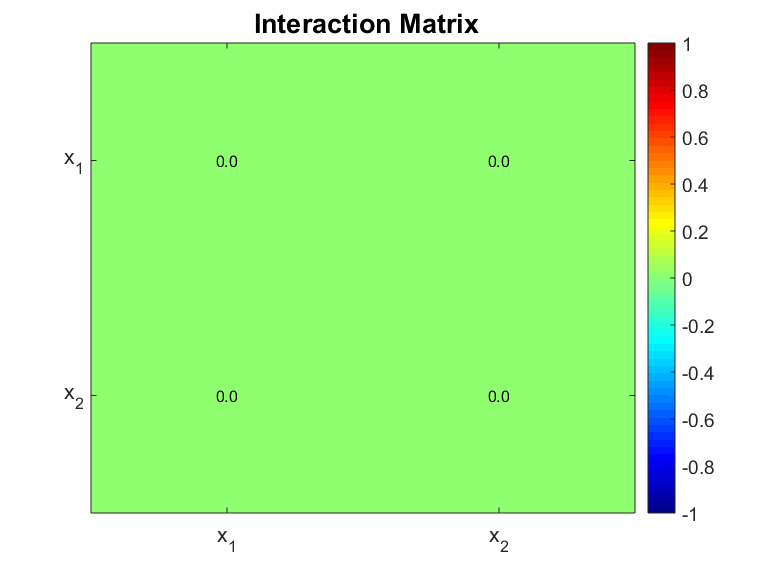
\includegraphics[width = \textwidth]{Stability/Interactions_case_study_1_no_interactions}
		\caption{Interaction matrix of model \eqref{system} with no interactions.}
		\label{case1_no_interactions}
	\end{subfigure}
	~
	\begin{subfigure}[b]{0.45\textwidth}
		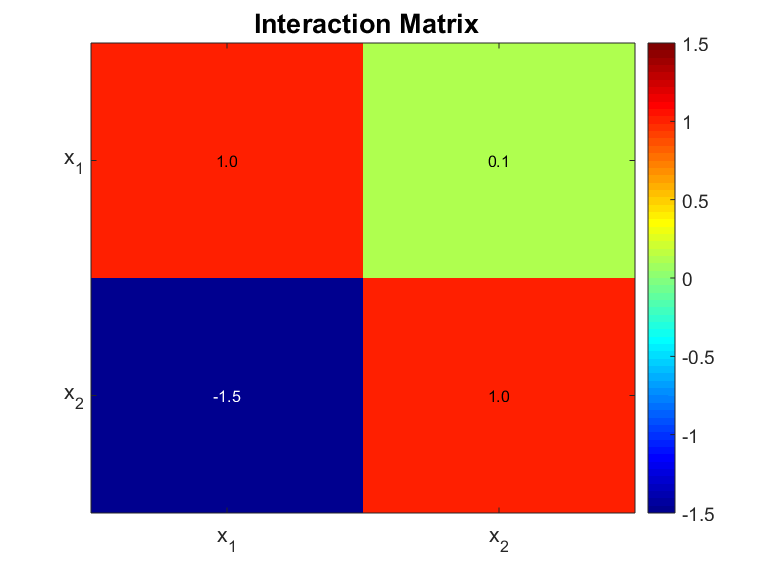
\includegraphics[width = \textwidth]{Stability/Interactions_case_study_1}
		\caption{Interaction matrix of model \eqref{system}.}
		\label{case1_interactions}
	\end{subfigure}
	\caption{Interaction matrices. Note how the presence of $x_1$ affects very negatively $x_2$ in \eqref{case1_interactions}. The sign of terms in the diagonal entries of the matrix represents interspecies interactions.}
\end{figure} 

\begin{figure}[h]
	\centering
	\begin{subfigure}[b]{0.45\textwidth}
		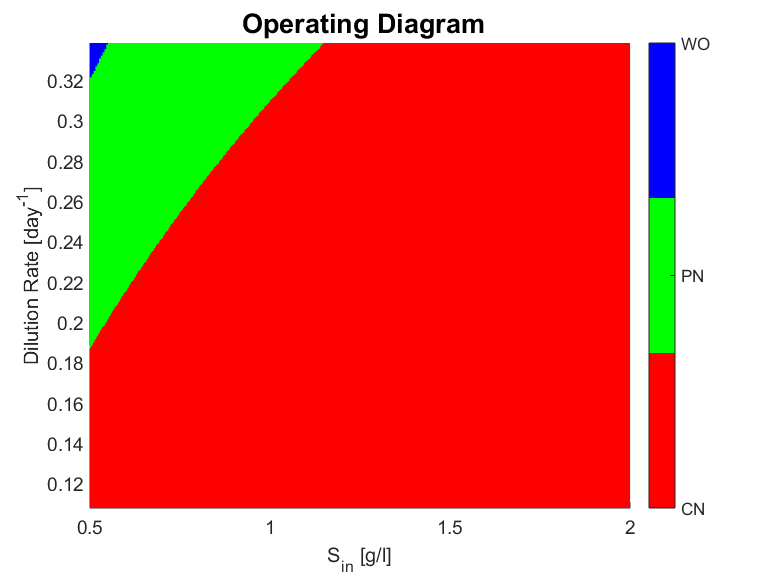
\includegraphics[width = \textwidth]{Stability/OD_case_study_1_no_interactions}
		\caption{Operating diagram of model \eqref{system} with no interactions (interaction matrix represented by \eqref{case1_no_interactions}).}
		\label{OD_no_interactions}
	\end{subfigure}
~
	\begin{subfigure}[b]{0.45\textwidth}
	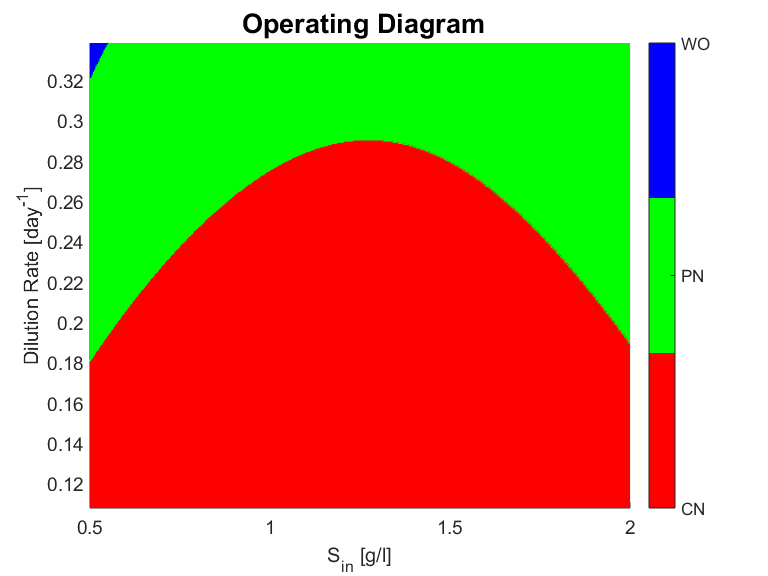
\includegraphics[width = \textwidth]{Stability/OD_case_study_1}
	\caption{Operating diagram of model \eqref{system} with interactions represented by \eqref{case1_interactions}.}
	\label{OD_interactions}
	\end{subfigure}
	\caption{Note how \ref{OD_interactions} has a much larger zone where partial nitrification takes place. This is due to the negative interaction $x_1$ plays against $x_2$.}
\end{figure} 
\clearpage

\textbf{Case study 2: 2 AOB and 2 NOB}

 The case study 2 is based on Dumont \textit{et al.}\cite{Dumont2016} model parameters. They proposed a distribution of parameters obtained from a Bayesian estimation method. Their fit describes well the dynamics of the two most abundant OTU in each functional group, but it still fails to capture the measured substrates dynamics. Kinetic parameters of case study 2 can be seen in table \ref{kinetic_parameters}. The estimated interaction matrix is shown in figure \ref{Interaction_1}. A second matrix is presented, which is obtained by the sign change of coefficient $a_{11}$ (figure \ref{Interaction_2}), and finally a third one is obtained by using a positive value for $a_{12}$ (figure \ref{Interaction_3}). 

\begin{table}[ht]
	\centering
	\begin{tabular}{|l|l|l|l|}
		\hline
		Case study 2 kinetic parameters & $\mu_i\,[1/day]$ & $K_i\,[mg/L]$ & $\frac{1}{y_i} \, [gr/gr]$ \\ \hline
		$x_1 \in G_1$ & 0.828  & 0.147 & 3.85  \\ \hline
		$x_2\in G_1$ &0.828   & 0.147 &  3.85\\ \hline
		$x_3\in G_2$ & 0.18 & 0.026 &  100 \\ \hline
		$x_4\in G_2$ & 0.18 & 0.026 &  100 \\ \hline
	\end{tabular}
	\caption{Kinetic parameters of model \eqref{system} from Dumont \textit{et al.} \cite{Dumont2016}}
	\label{kinetic_parameters}
\end{table}

\begin{figure}[h]
\begin{subfigure}[b]{0.32\textwidth}
	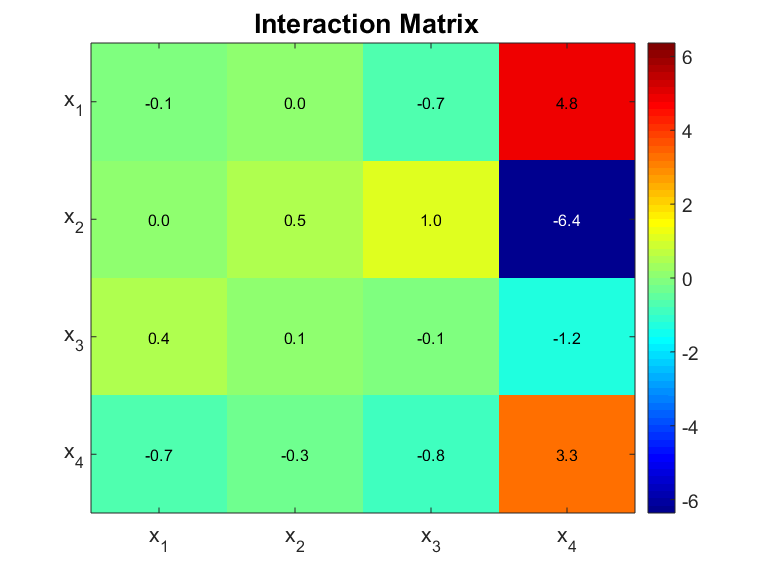
\includegraphics[width=\textwidth]{Stability/Interactions_parameters_Dumont}
	\caption{Originally calibrated interaction matrix.}
	\label{Interaction_1}
\end{subfigure}
~
\begin{subfigure}[b]{0.32\textwidth}
	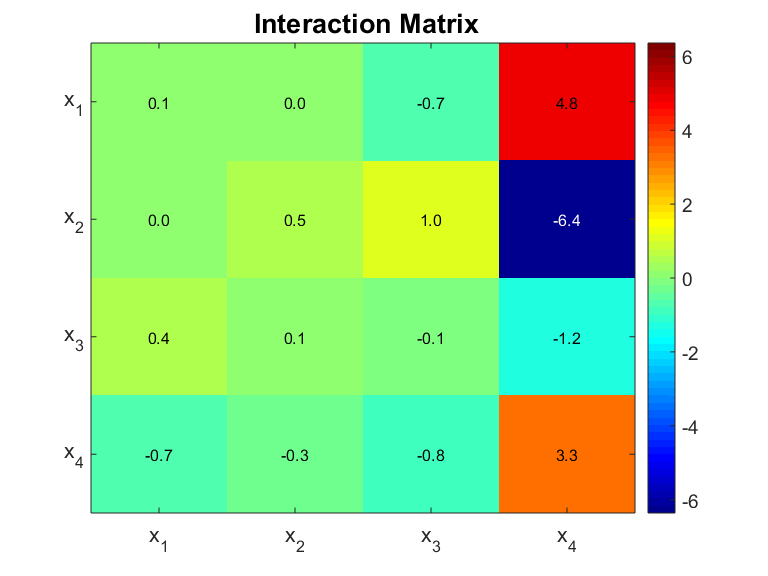
\includegraphics[width=\textwidth]{Stability/Interactions_parameters_modified}
	\caption{Modified interaction matrix with positive intraspecies interaction $a_{11}>0$.}
	\label{Interaction_2}
\end{subfigure}
~
\begin{subfigure}[b]{0.32\textwidth}
	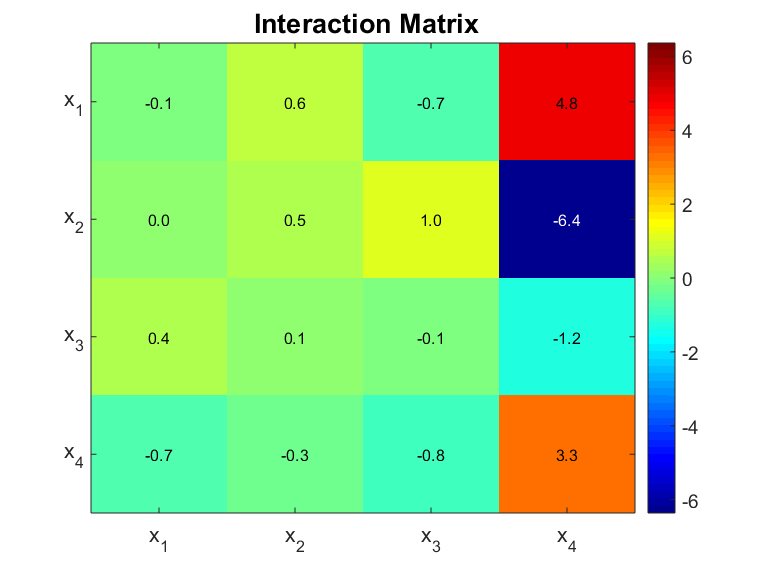
\includegraphics[width=\textwidth]{Stability/Interactions_parameters_modified_2}
	\caption{Modified interaction matrix with positive interspecies interaction  $a_{12}>0$.}
	\label{Interaction_3}
\end{subfigure}
	\caption{Interaction matrices for each case for a consortia of 4 bacterial species where $x_1$ and $x_2$ are AOB and $x_3$ and $x_4$ are NOB. Parameters $a_{11}$ and $a_{12}$ were modified in figures \eqref{Interaction_2} and \eqref{Interaction_3}, respectively.}
	\label{Interactions}
\end{figure} 


\begin{figure}[ht]
	\centering
	\begin{subfigure}[b]{0.32\textwidth}
	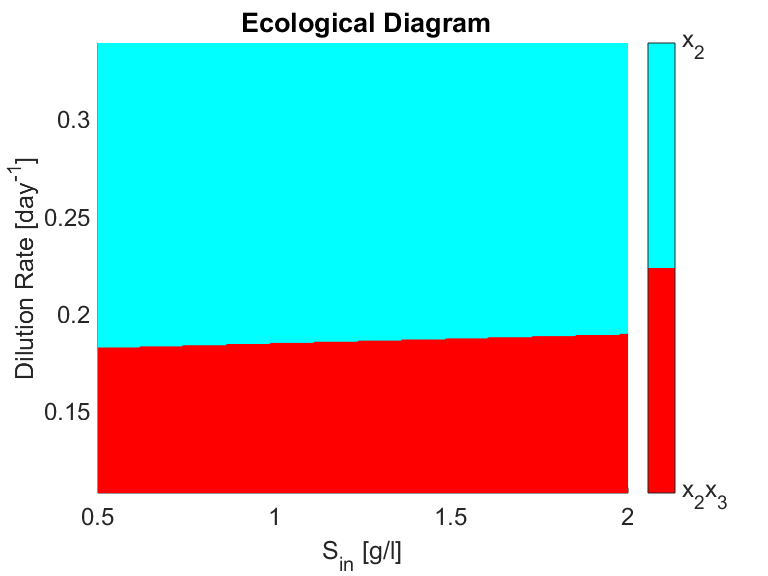
\includegraphics[width=\textwidth]{Stability/ED_parameters_Dumont}
	\caption{Original parameters ecological diagram.}
	\label{ED 1}
	\end{subfigure}
~
	\begin{subfigure}[b]{0.32\textwidth}
	\includegraphics[width=\textwidth]{Stability/ED_parameters_modified}
	\caption{Modified interaction matrix ecological diagram.}
	\label{ED 2}
	\end{subfigure}
~
\begin{subfigure}[b]{0.32\textwidth}
	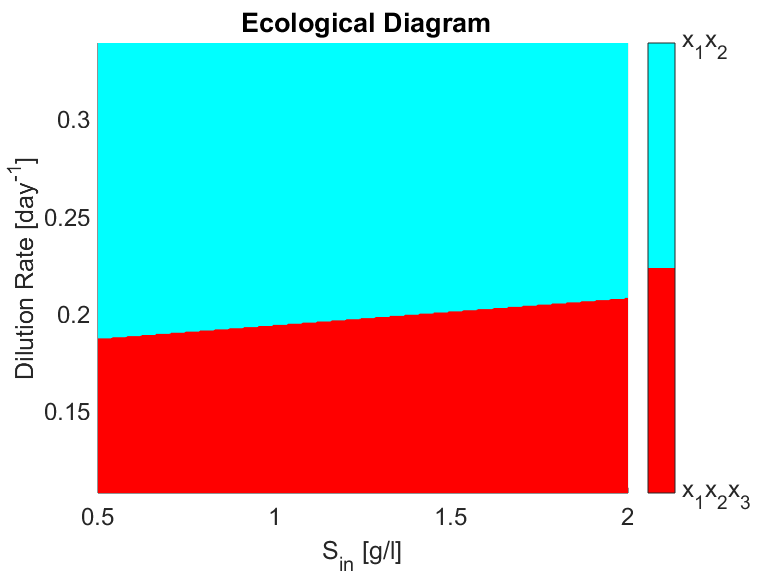
\includegraphics[width=\textwidth]{Stability/ED_parameters_modified_2}
	\caption{Modified interaction matrix ecological diagram.}
	\label{ED 3}
\end{subfigure}

	\caption{Ecological diagrams for both cases. The different zones represent the combination of surviving species in the steady state. PN takes place when neither $x_3$ nor $x_4$ are present. Note that in figure \ref{ED 2} two stable equilibria exist for each zone. CN takes place if $x_3$ or $x_4$ are present. }
	\label{ecological_diagrams}
\end{figure}

The ecological diagrams are presented in figure \ref{ecological_diagrams}. Comparing figure \ref{ED 1} with \ref{ED 2} one can see a very different situation. Note how every zone in figure \ref{ED 2} has two stable equilibria, meaning that the outcome of the system is strongly determined by its initial conditions, particularly interesting is the green zone where either $x_1,x_3$ coexist or $x_2$ alone remains, because in operational terms this means that either PN or CN may take place.

One can see that coexistence in the same functional group is never attained in figure \ref{ED 1}, whereas in figure \ref{ED 2} $x_1$ and $x_2$, both AOB, coexist in either partial or complete nitrification. That means that the model is able to overcome the competitive exclusion principle \cite{lobry2017chemostat} (CEP) paradigm. The CEP roughly states that if two species are growing on the same limiting resource, and their growth laws only depend non decreasingly on the resource, then only one of them will survive in the long run. This is interesting in light of reports on wastewater treatment plants where coexistence between species in nitrifying reactors has been shown \cite{Wagner2002}, thus implying that a more complex growth law (as shown in here) or model structure involving other biological processes is required to include microbial diversity in mathematical models. 

\subsection{Remarks}

The model here presented serves to illustrate that by considering a more complex growth rate that tries to model ecological interactions one might explain differences in reactors operating under similar conditions. It also shows a new mechanism by which the CEP no longer holds and where multiple stable equilibria may appear. Since the gLV model discussed (and calibrated in \cite{Dumont2016}) fails to completely capture the dynamics observed in the chemostat experiments, the next section proposes a new model to study interactions.


\section{Generalized approach for modelling interactions}
In the previous sections interactions were modelled as an affine function of the OTU concentration that multiplies a substrate dependent growth equation. More generally the interaction function represents how the growth rate of species $i$ is affected by the concentration of other species, $x$: 

Given a vector $(v_1,\dots,v_n)^\top$ the interaction function $\I$ is noted as:
\begin{align}
\begin{array}{rc}
\I: \R_+^n \rightarrow & \R_+^n\\
& \\
v \rightarrow & \begin{pmatrix}
I_1(v) \\
I_2(v) \\ 
\vdots  \\
I_n(v)
\end{pmatrix}
\end{array}
\end{align}

Let $f_i(s)$ be a bounded, positive, and continuous function of $s$ (e.g. Monod, Haldane). The growth equation of OTU $i$ becomes:
\begin{align}
	\mu_i(s,x) = f_i(s)I_i(x)
\end{align}
Note $f(s) := (f_1(s),\dots,f_n(s))^\top$.
	\label{growthForm}

Since the growth of a single strain in batch experiments is driven by the substrate concentration, when no interactions are present one should recover expression $f_i(s)$. Therefore if there are no interactions then $I_i(x) = 1$. From this hypothesis, note that $ \lim \limits_{x \rightarrow 0} I_i(x) = 1$ since if there is minimal presence of OTU, interactions can not exist. Furthermore for this study it is assumed that $I_i(\cdot)$ is a continuously differentiable function on $x$. For making explicit all of the former:

\begin{hypo}
	The interaction function $\I$ previously defined satisfies:
	\begin{enumerate}
		\item\begin{align}
		\I \left( (0,\dots,0)^\top \right) = 
		(1,\dots,1)^\top 
		\end{align}
		\item Let $\Omega$ be an open subset of $ \R^n $ then $\I \in C^1(\Omega)$.
	\end{enumerate} 
\end{hypo}


Note $J_I(x)$ the Jacobian matrix of function $\mathcal{I}$, then a first order approximation of $\I(\cdot)$ centred at $\bar{x}$ gives: $\I(x) = \I(\bar{x}) + J_I(\bar{x})(x-\bar{x}) + o(\Vert x- \bar{x} \Vert)$. When $\bar{x}= 0$ one recovers the growth expression from the previous section (equations \eqref{gLV growth1} and \eqref{gLV growth2}) implying that $J_I(\bar{0})$ can be seen as the interaction matrix from model \eqref{system}.

\subsection{Unravelling the Interaction Function}

Suppose that the functions $f_i(s)$, and the yields $y_i$ are well-known. By using experimental measurements of $x$, represented by $z(t)$, the objective is to reconstruct function $I(x)$. For doing so, the terms $I_i(x)$ are replaced by controls $u_i(t)$, thus $I_i(x(t)) = u_i(t)$. A control law is obtained by solving a nonlinear optimal tracking problem.	

Consider the observable system \eqref{Controlsystem} ($y(t) = x(t)$ being the observer) where $g(\cdot)$ is a known function.

\begin{align} 
\label{Controlsystem}
\begin{array}{cl}
\dot{x_i} =& \left(f_i(s)u_i(t) -D \right)x_i \quad \forall i \in G_1\\
\dot{x_i} =& \left(f_i(s)u_i(t) -D \right)x_i \quad \forall i \in G_2\\
\dot{s_1} =& \displaystyle (s_{in}-s_1)D-\sum\limits_{i \in G_1}\frac{1}{y_i}f_i(s)u_i(t) x_i  \\
\dot{s_2} = & \displaystyle -s_2D+\sum\limits_{i \in G_1}\frac{1}{y_i}f_i(s)u_i(t)	-\sum\limits_{i \in G_2}\frac{1}{y_i}f_i(s)u_i(t) x_i  \\
\dot{s_3} =&  \displaystyle -s_3D+\sum\limits_{i \in G_2}\frac{1}{y_i}f_i(s)u_i(t) x_i \\
y(t) & = x
\end{array}
\end{align}	

For this model $g(x,s) = x$, since we are observing measurements coming from genetic sequencing. Consider the weighted norms defined by positive definite matrices $Q$ and $R$, represented by $\Vert \cdot \Vert_Q$ and $\Vert \cdot \Vert_R$, respectively, and a positive real $\bar{u}$. The optimal tracking problem is defined as: 

\begin{align}
\label{Optimal Control} \begin{array}{cc} \min &  \int \limits_{0}^{T} \Vert g(x,s) - z \Vert_Q + \Vert(u -\vec{1}) \Vert_R dt\\
s.t.& 
(x,s_1,s_2,s_3)\mbox{ solution of \eqref{Controlsystem}} \\
&u_i(t) \in [0,\bar{u}]
\end{array}	
\end{align} 

The control $u(t)$ is intended to drive the system to be near a desired output $z(t)$, which in this context are the measurements of the concentrations of OTU. The term $\Vert(u -\vec{1}) \Vert_R$, was added for two reasons:
\begin{itemize}
\item First because the interest is testing the idea that interactions could be driving the system. Therefore adding a penalization in the objective function for each control to remain near $1$ can be seen as an attempt to explain data without any interaction.
\item Second, to force a regularized control. Otherwise note that $u$ is linear in \eqref{Controlsystem}, therefore if the integral cost does not have a non-linear expression of $u$ the optimal control will be of a bang-bang type with possibly singular arcs \cite{harmand2019optimal}. Since the objective is to find a differentiable expression of $I(x)$ the addition of the regularization term is deemed necessary.
\end{itemize} 
The problem of approximating the solution of the system to a desired reference ($z$ in this case) is called the optimal tracking problem. For solving such a problem the approach developed by Cimen \textit{et al.} \cite{Cimen2004, Cimen2008} was adapted to our problem. The method proposed involves the resolution of Approximating Sequences of Ricatti Equations (ASRE). 

The method consists on iteratively calculating trajectories of system \eqref{Controlsystem} with a certain control and feeding a non-autonomous Ricatti differential equation with the resulting trajectory. Then a control law that uses the solution of the Ricatti equation is proposed and a new trajectory is calculated. The iteration is stopped when a convergence in the output or  the control is observed.

The tracking problem does not consider a constrained control. Nevertheless, the methods of Cimen \textit{et al.}\cite{Cimen2004} were directly used with an explicit constraint in the synthesis of the control. Even though this is probably suboptimal when the control reaches its bounds, one at least is certain of its optimality when the control never reaches its constraints.

Another departure from their method is that in their formulation an approximation of the dynamics for calculating the trajectories is used. They proved that such a linearisation converged to the original dynamics. In the case here presented the linearisation of the dynamics was not necessary.

The change of variable $u_i(t) = v_i(t) + 1$ is used for technical reasons explained in the supplementary material section. This in turn implies $v_i(t) \in [-1,\bar{u}-1]$.

The feedback control $v(t)$, will be of the form $v(t) = -R^{-1}\tilde{B}^\top(t)\left(\tilde{P}(t)x(t)-s_f(t)\right)$. Where matrix $P(t)$ and vector $s_f(t)$ solve differential equations. In the appendix it is proved that because of the structure of the system one only needs to calculate $2n$ differential equations for the synthesis of the control, instead of $(n+3)^2 + (n+3)$ that would imply the direct application of the method. Which renders the method- at least theoretically- scalable for a growing number of OTU.

\subsection{Proof of concept}

The approach was tested against synthetic data generated by simulating model \eqref{system} using the parameters of the case study 1 (table \ref{kinetic_parameters_case_study_1}) with interaction matrix given by \eqref{case1_interactions}. In the operating diagram of the same case (figure \eqref{OD_interactions}) the red zone implies complete nitrification, while the green zone means partial nitrification. For integrating the former phenomena in the simulation, the system was simulated for 300 days, and perturbed at day 150 from the CN zone ($(s_{in},D) = (1.25,0.22)$) to a PN zone ($(s_{in},D) = (1.95,0.22)$). Simulations can be seen in figure \ref{synthetic_data}. Note how from day 150 the NOB population represented in figure \eqref{PC_synthetic_NOB} decreases, which in turn implies a decrease in $s_3$, as seen in figure \eqref{PC_synthetic_metabolites}.


\begin{figure}[h]
	\centering
	\begin{subfigure}{0.32 \linewidth}
	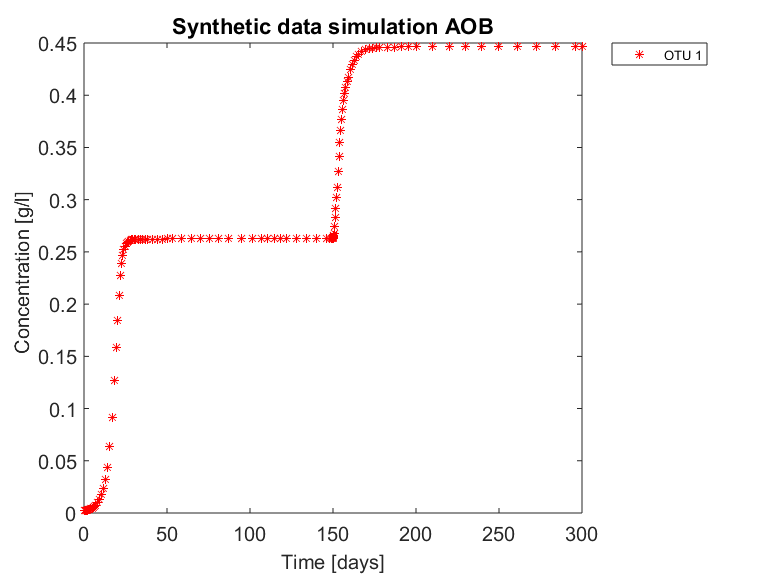
\includegraphics[width=\linewidth]{proof_of_concept/250309_POC_AOB_plot}
	\caption{AOB.}
	\label{PC_synthetic_AOB}
	\end{subfigure}
	\begin{subfigure}{0.32 \linewidth}
	\centering
	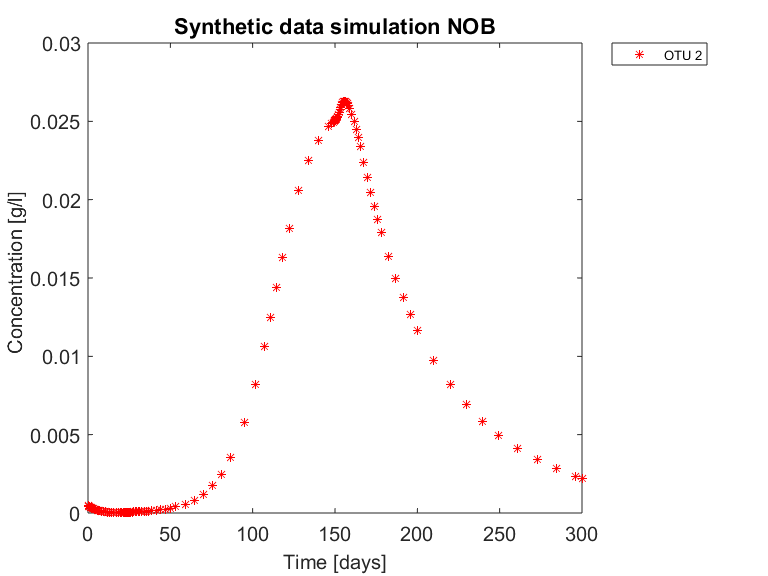
\includegraphics[width=\linewidth]{proof_of_concept/250309_POC_NOB_plot}
	\caption{NOB.}
	\label{PC_synthetic_NOB}
	\end{subfigure}
	\begin{subfigure}{0.32 \linewidth}
	\centering
	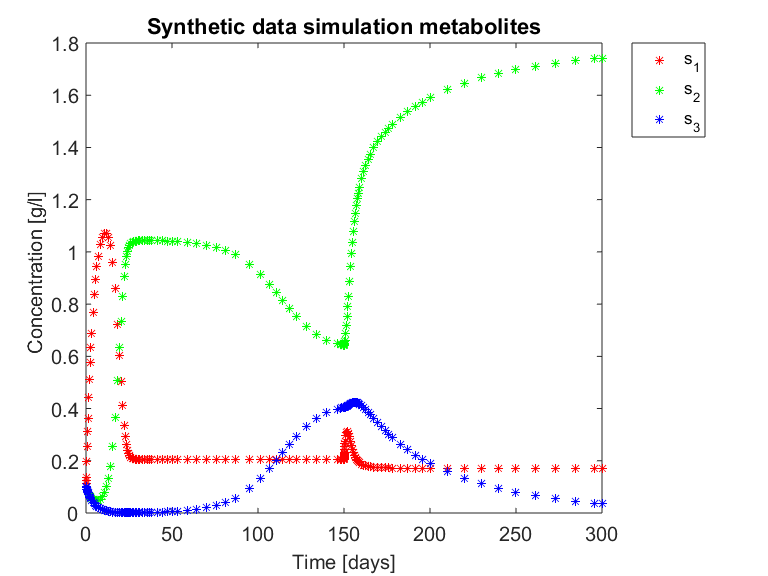
\includegraphics[width=\linewidth]{proof_of_concept/250309_POC_metabolites}
	\caption{Metabolites.}
	\label{PC_synthetic_metabolites}
	\end{subfigure}
	\caption{Synthetic data generated by model \eqref{system}, with parameters from case study 1. Note the effects of the increased input $s_{in}$ generated in day 150.}
	\label{synthetic_data}
\end{figure}





%For applying the optimal tracking approach, the choice of matrices $Q$ and $R$ are always of discussion in a quadratic regulator. $Q$ represents the covariance matrix of measurements, while $R$ is subject to interpretations depending on the context: in the case here presented it does not have \textit{a priori} definite meaning. For gaining some insight, its behaviour is studied when $\rho(R) \rightarrow 0$, with $\rho(R)$ being the spectral radius of matrix $R$. In the simulations here presented $Q = I_n$ and $R = \lambda I_n$. In the supplementary material section. $\lambda$ is varied from $10^{-1}$ to $10^{-7}$. The case $\lambda = 10^{-4}$ is shown in here for discussion. 

 For the tracking procedure the functions $f_i(s)$ and the yields $y_i$ were the same as those used for simulating the synthetic data (parameters in table \ref{kinetic_parameters_case_study_1}) and the control is meant to account for the interaction term. The $Q$ and $R$ matrices are $\lambda I_n$ and $I_n$, respectively, with $\lambda = 10^{-4}$. The results of the procedure to identify interactions can be seen in figure in figure \ref{POC_tracking}. Figures \ref{PC_total_biomass}, \ref{PC_AOB}, and \ref{PC_NOB} show the total biomass concentration, and the trajectories for the OTU belonging to $G_1$ and $G_2$, respectively. It can be seen that the method approaches well the trajectories of the OTU, with a better result for the AOB community, which can be explained by the one order of magnitude difference in their concentrations (which in turn is a consequence of the one order of magnitude difference in their yields). The metabolites concentration represented in figure \ref{PC_metabolites} are in accordance with the simulated: The method is able to reconstruct the metabolites trajectories from the community measurements. 


\begin{figure}[h]
	\centering
	\begin{subfigure}{0.45 \linewidth}
	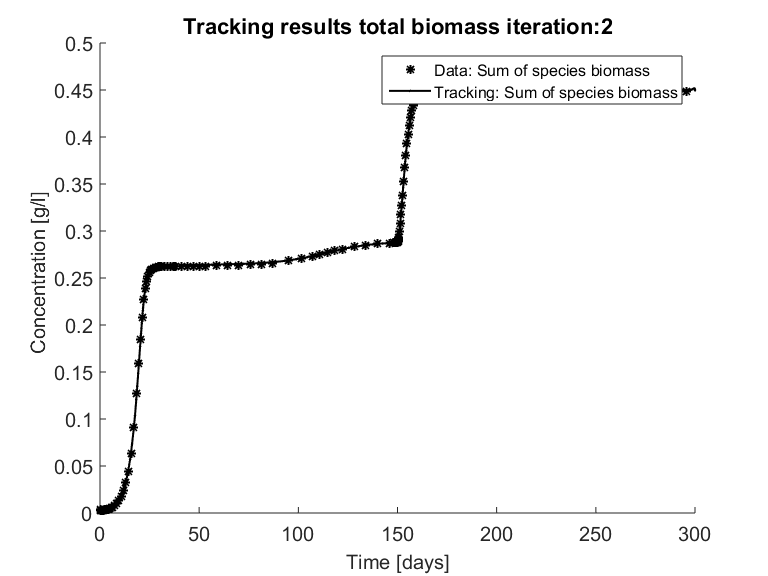
\includegraphics[width= \textwidth]{proof_of_concept/250309_POC_try3_iter_2_Biomass}
	\caption{Total biomass.}
	\label{PC_total_biomass}
	\end{subfigure}
~
	\begin{subfigure}{0.45 \linewidth}
		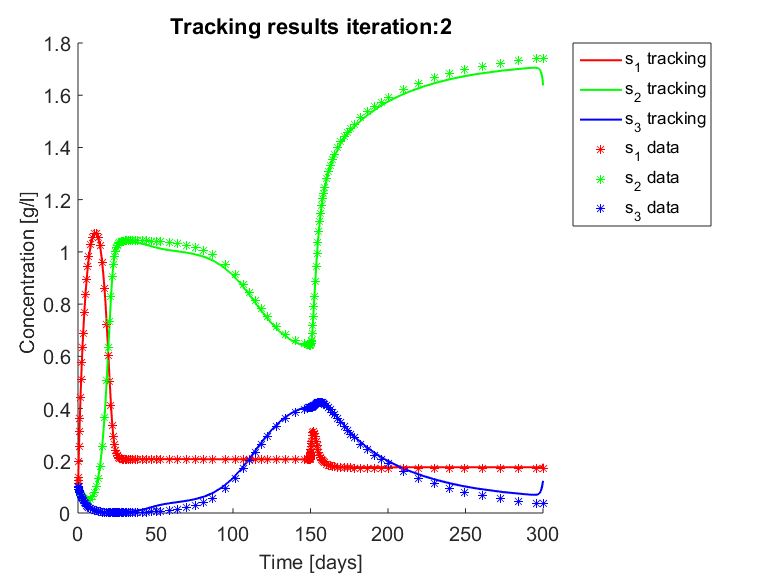
\includegraphics[width=\textwidth]{proof_of_concept/250309_POC_try3_iter_2_metabolites}
		\caption{Metabolites. }
		\label{PC_metabolites}
	\end{subfigure}

	\begin{subfigure}{0.45 \linewidth}
		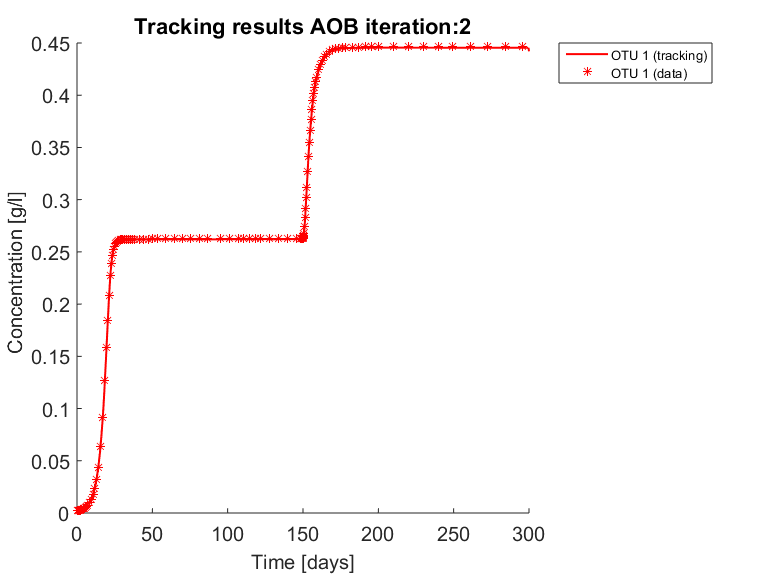
\includegraphics[width=\textwidth]{proof_of_concept/250309_POC_try3_iter_2_AOB_plot_1}
		\caption{AOB biomass.}
		\label{PC_AOB}
	\end{subfigure}
	~
	\begin{subfigure}{0.45 \linewidth}
		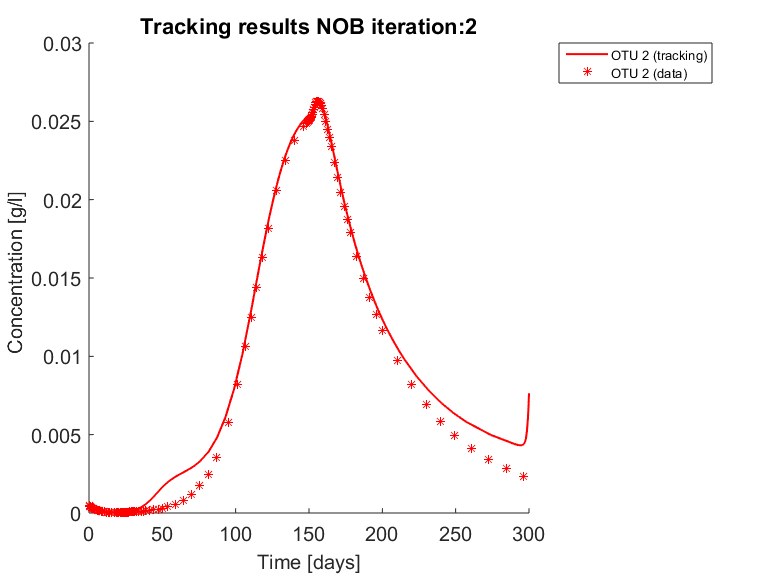
\includegraphics[width=\textwidth]{proof_of_concept/250309_POC_try3_iter_2_NOB_plot_1}
		\caption{NOB biomass. }
		\label{PC_NOB}
	\end{subfigure}
\caption{Asterisks represent the synthetic data, while the continuous lines represent the method's output. The method is able to reconstruct the metabolites pattern, from the biomasses concentrations.}
\label{POC_tracking}
\end{figure}



Figure \ref{POC_control} shows the controls and the corrected growth rate for each functional group. The control for each funcional group can be seen in figures \ref{Control AOB no noise} and \eqref{Control NOB no noise}. Note that from the structure of a quadratic regulator, since there is no cost in the final state, the end value is always 1. Figures \ref{AOB_growth_POC} and \ref{NOB_growth_POC} show the resulting growth rates for $AOB$ and $NOB$, respectively, without the control $u_i(t)$. Figures \ref{AOB_growth_control_POC} and \ref{NOB_growth_control_POC} are the complete expression that determines growth rate, that is  $f_i(s(t))u_i(t)x_i(t)$. Note how little the shape changes with respect to figures \ref{AOB_growth_POC} and \ref{NOB_growth_POC}, which might mislead the reader to conclude that the control had reduced effects in the dynamics. The way out of this conundrum is to remember that the control's effects are already included in $x_i(t)$ and $s_i(t)$, and thus in expression $f_i(s(t))x_i(t)$. 

\begin{figure}[h]
	\centering
	\begin{subfigure}{0.45 \linewidth}
		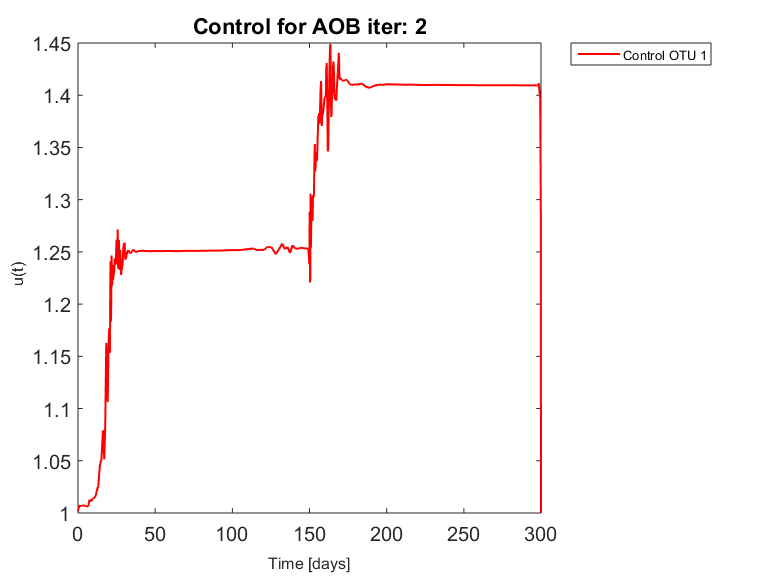
\includegraphics[width=\linewidth]{proof_of_concept/250309_POC_try3_iter_2_Control_AOB_plot_1}
	\caption{Control for the AOB population.}
	\label{Control AOB no noise}
	\end{subfigure}
	\begin{subfigure}{0.45 \linewidth}
		\centering
		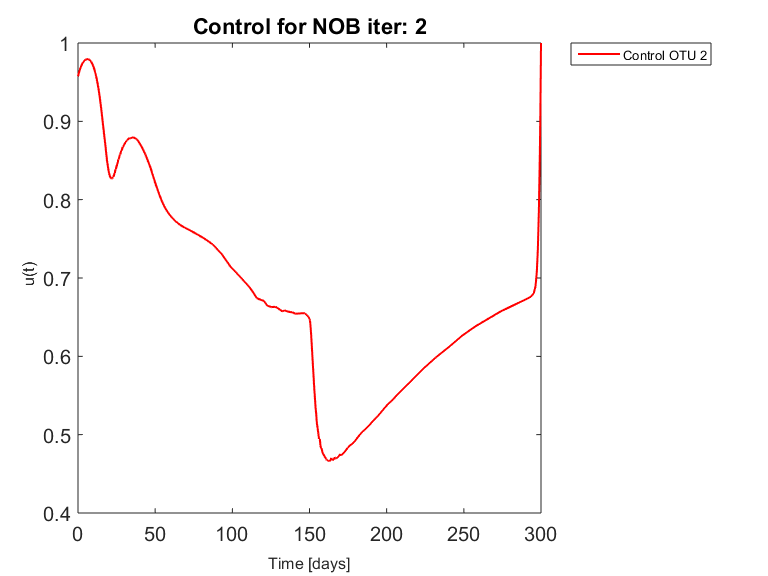
\includegraphics[width=\linewidth]{proof_of_concept/250309_POC_try3_iter_2_Control_NOB_plot_1}
	\caption{Control for the NOB population.}
	\label{Control NOB no noise}
	\end{subfigure}

	\begin{subfigure}{0.45 \linewidth}
		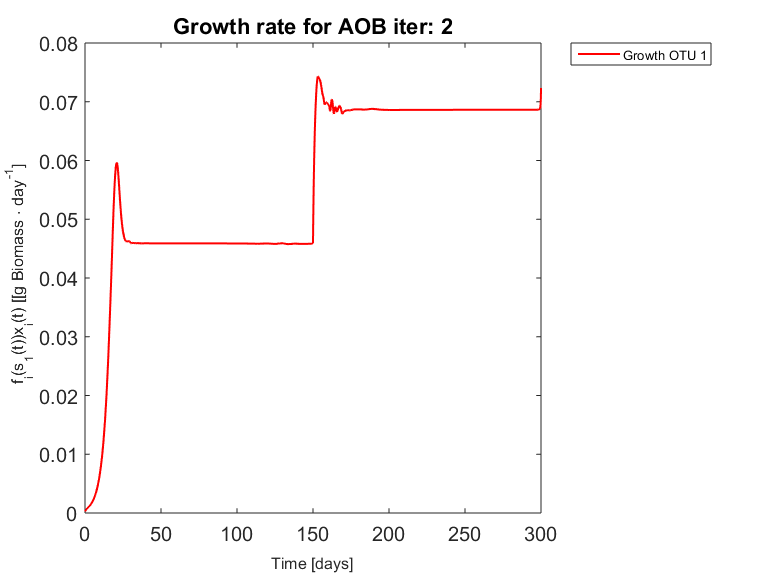
\includegraphics[width=\linewidth]{proof_of_concept/250309_POC_try3_iter_2_growth_AOB_plot_1}
		\caption{Growth rate of the model for AOB community.}
		\label{AOB_growth_POC}
	\end{subfigure}
	\begin{subfigure}{0.45 \linewidth}
		\centering
		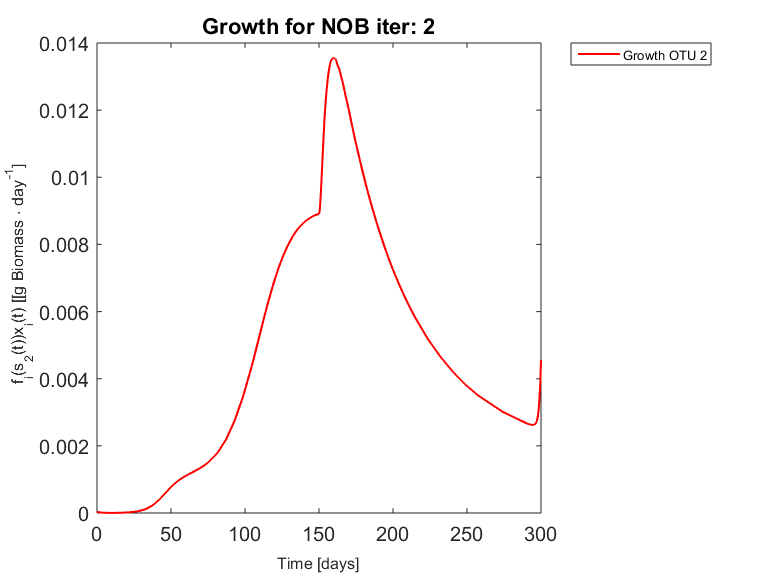
\includegraphics[width=\linewidth]{proof_of_concept/250309_POC_try3_iter_2_growth_NOB_plot_1}
	\caption{Growth rate of the model for the NOB community.}
	\label{NOB_growth_POC}
	\end{subfigure}

	\begin{subfigure}{0.45 \linewidth}
		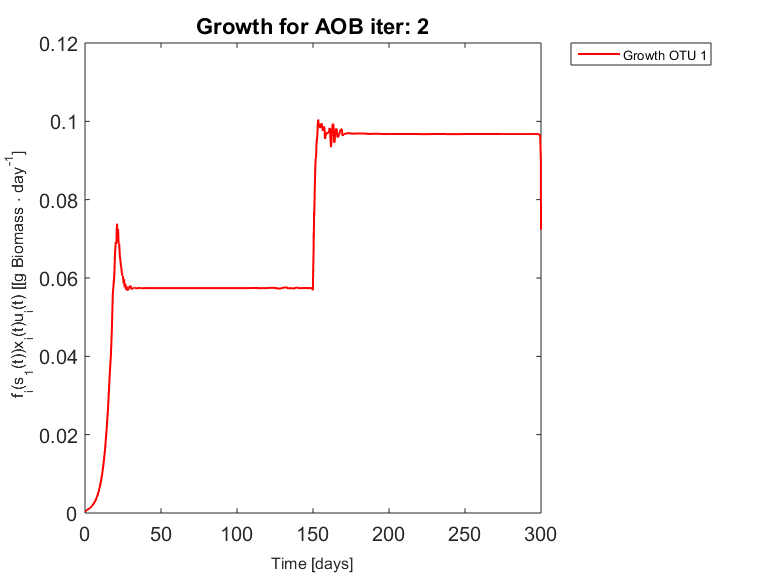
\includegraphics[width=\linewidth]{proof_of_concept/250309_POC_try3_iter_2_growth_control_AOB_plot_1}
		\caption{Growth rate of the model for AOB community.}
		\label{AOB_growth_control_POC}
	\end{subfigure}
	\begin{subfigure}{0.45 \linewidth}
		\centering
		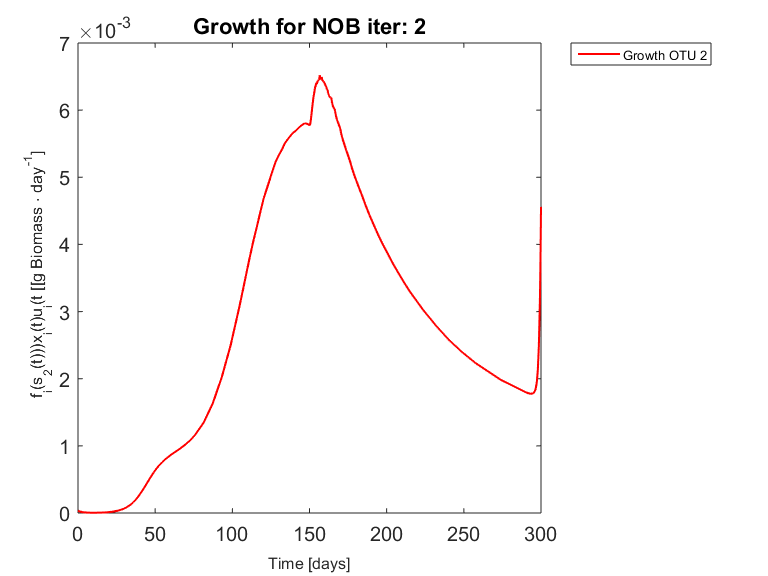
\includegraphics[width=\linewidth]{proof_of_concept/250309_POC_try3_iter_2_growth_control_NOB_plot_1}
		\caption{Growth rate of the model for the NOB community.}
		\label{NOB_growth_control_POC}
	\end{subfigure}
	\caption{Control and growth rates resulting from the tracking approach.}
	\label{POC_control}
\end{figure}

%In figure \ref{Comparison_lambda} the different controls obtained by varying $\lambda$ for two species are compared to the interaction function simulated that is $1+A(x(t))$, where $x(t)$ is the synthetic data. One can see that due to this property of the end value becoming 1, the two do not coincide, however, when $\lambda$ is decreased one can see that the control roughly approaches the respective interaction function at the cost of very sharp changes.

%\begin{figure}[h]
%	\centering
%	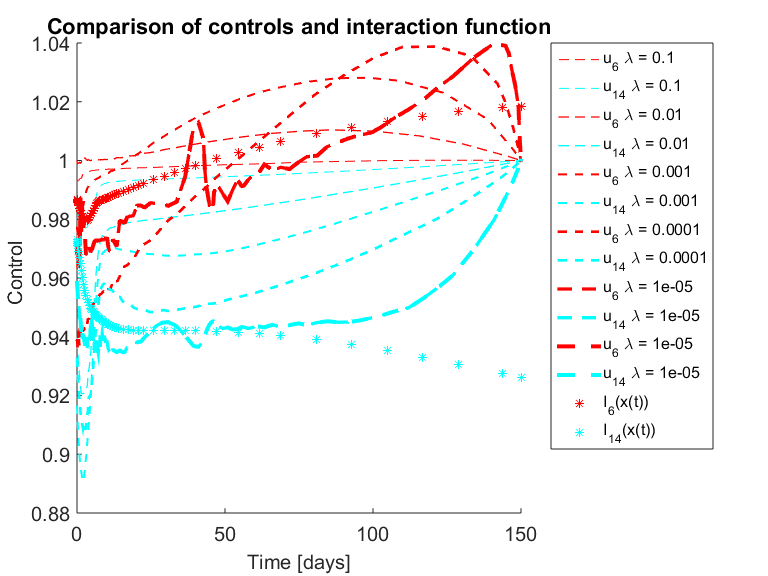
\includegraphics[width=0.5\textwidth]{Synthetic_data//Comparison_different_control}
%	\caption{Obtained controled for different $\lambda$ for two OTU and the interaction function used in the simulation of synthetic data.}
%	\label{Comparison_lambda}
%\end{figure}

\clearpage
\section{Application}
 
%The method was stopped after 10 iterations where each iteration took approximately 800 seconds of computing time in a computer equipped with 8gb of RAM memory and Intel core i3-7100U CPU 2,40 GHz.\iffalse Cette phrase devrait figurer dans la partie précédente ?\fi

The tracking problem was applied to data coming from a nitrification process; the experimental conditions are described in \cite{dumont2008observers}. For exploring the hypothesis of interactions as drivers of bioreactors performance environmental conditions should be kept as constant as possible. Therefore only data from day $183$ onwards was used because a change in the operating temperature happened at that point, which is known to have an effect on kinetics. For choosing which species belong in which functional group, the procedure described in \cite{Ugalde-Salas2019} was used: from day $183$ to day $315$: 31 OTU were identified in the $G_1$ group (AOB) and 5 in the $G_2$ functional group (NOB). 


\begin{table}[ht]
	\centering
	\begin{tabular}{|l|l|l|l|}
		\hline
		Kinetic Parameters & $\mu_i\,[1/day]$ & $K_i\,[g/L]$ & $\frac{1}{y_i} \, [gr/gr]$ \\ \hline
		$x_1 \in G_1$ & 1.97  & $7\cdot 10^{-1}$ & 4.49  \\ \hline
		$x_2\in G_2$ & 1.87 & $5.4\cdot 10^{-1}$ &  45.51 \\ \hline
	\end{tabular}	
	\caption{A set of kinetic parameters of model \eqref{system}.}
	\label{kinetic_parameters_application}
\end{table}



A first example of the procedure is performed when the classified OTU are regrouped in their assigned functional groups by adding their concentrations. A 5 dimensional dynamical system is obtained. The same procedure is applied where no regrouping occurs and the system state grows to 39. 

The knowledge of functions $f_i(s)$ was based on a study of nitrification's kinetic parameters\cite{Wiesmann1994}. Particularly given the system's ammonium and nitrate concentration a Monod function (eq \eqref{monod}) was used for $G_1$ and $G_2$ with parameters given in table \ref{kinetic_parameters_application}. The yields were fitted to match the nitrogen mass balances. In this case the $Q$ and $R$ matrices were $\begin{bmatrix}
\lambda_1 I_{n_1} &0  \\ 0& \lambda_2 I_{n_2}
\end{bmatrix}$ and $I_n$, respectively, with $\lambda_1 = 10^{-4}$ and $\lambda_2 = 10^{-5}$ in order to better track the NOB trajectories.

\begin{align}
\label{monod} f_i(s) &= \bar{\mu}_2 \dfrac{s_1}{K_1 +s_1} \, \forall i \in G_1 \\
\notag  f_i(s) &= \bar{\mu}_2 \dfrac{s_2}{K_2 +s_2 } \, \forall i \in G_2
\end{align}

For the reader to gain understanding of the situation, a simulation of the system using the experiments operating parameters ($D$ and $s_{in}$) is presented without control (i.e. $u(t)= 1$) in  figure \ref{u=1 simulation.}. $s_3$ accumulates all along the trajectory, but when compared to data it is clear that $s_3$ stops accumulating after a while. 

\begin{figure}[h]
	\centering	
	\begin{subfigure}{0.45 \textwidth}
		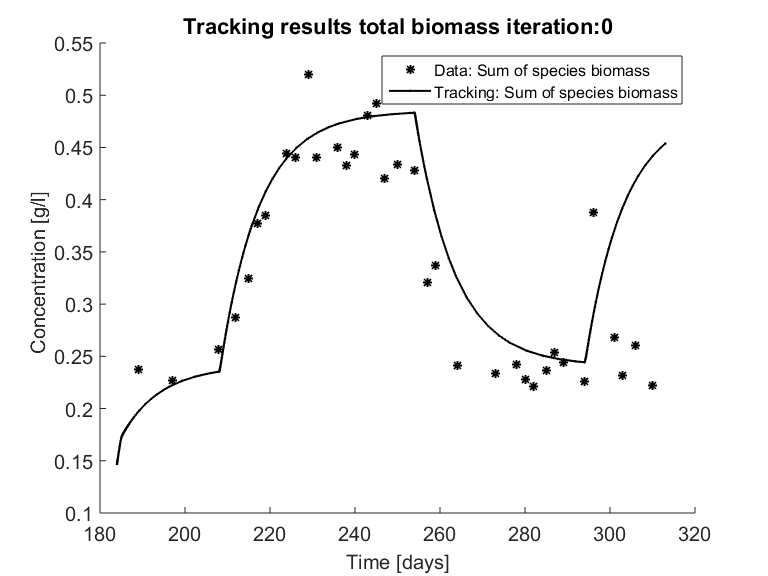
\includegraphics[width=\textwidth]{Application//191218_Reactor_A_Biomass_iter_0}
		\caption{Total Biomass.}
		\label{biomass_no_control}
	\end{subfigure}
	\begin{subfigure}{0.45 \textwidth}
		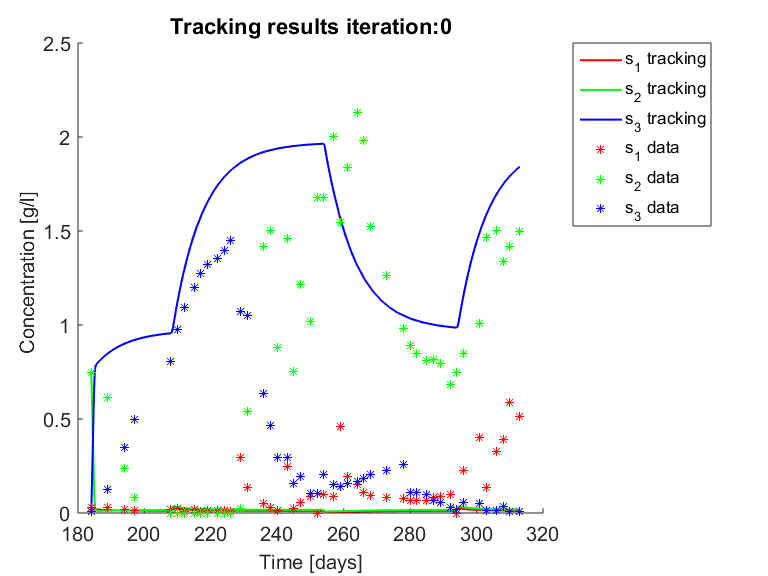
\includegraphics[width= \textwidth]{Application//191218_Reactor_A_metabolites_Iter_0}
		\caption{Metabolites.}
		\label{u=1_metabolites}
	\end{subfigure}
		\caption{Simulation of system \eqref{Controlsystem} when $u=1$, with functions as in \eqref{monod}. Data points are represented by a star. The continuous line represents the simulation.}
		\label{u=1 simulation.}
\end{figure}



\begin{figure}[h]
	\centering
	\begin{subfigure}{0.45 \linewidth}
		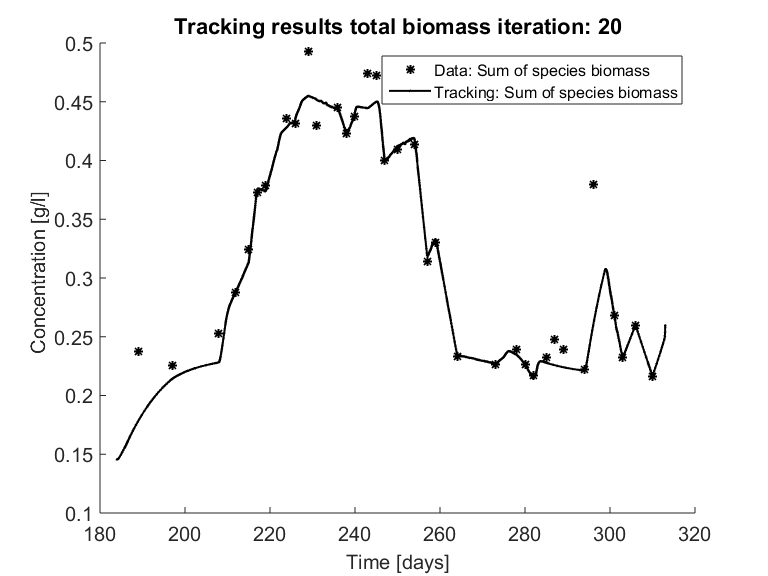
\includegraphics[width= \textwidth]{Application/200407_regroup_OTU_try2_iter_20_Biomass}
		\caption{Total Biomass.}
		\label{Total Biomass application}
	\end{subfigure}
	~
	\begin{subfigure}{0.45 \linewidth}
		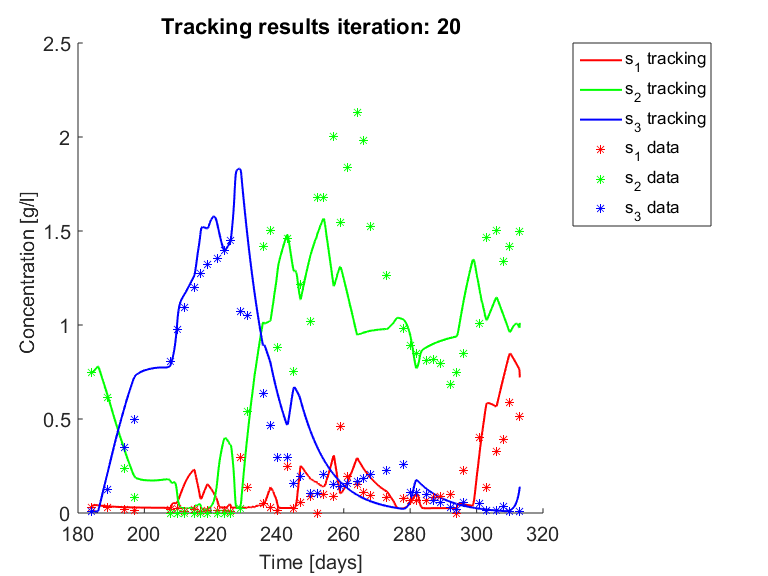
\includegraphics[width=\textwidth]{Application/200407_regroup_OTU_try2_iter_20_metabolites}
		\caption{Metabolites.}
		\label{Metabolites application}
	\end{subfigure}
	\begin{subfigure}{0.45 \linewidth}
		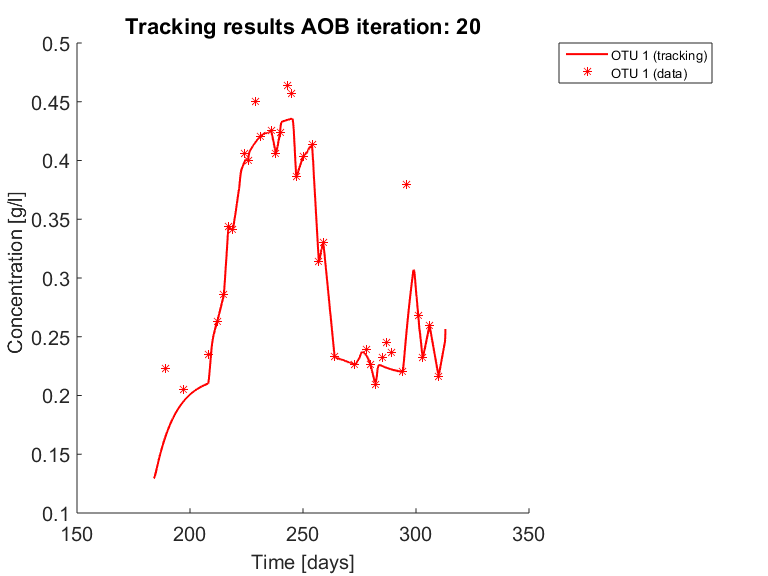
\includegraphics[width=\textwidth]{Application/200407_regroup_OTU_try2_iter_20_AOB_plot_1}
		\caption{AOB biomass.}
		\label{AOB application}
	\end{subfigure}
	~
	\begin{subfigure}{0.45 \linewidth}
		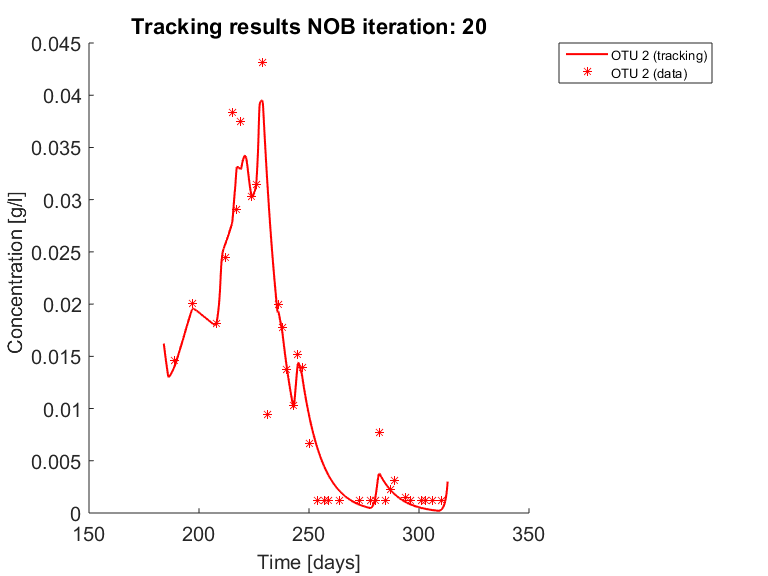
\includegraphics[width=\textwidth]{Application/200407_regroup_OTU_try2_iter_20_NOB_plot_1}
		\caption{NOB biomass.}
		\label{NOB application}
	\end{subfigure}
\caption{Results on applying the tracking method to a nitrification experiment when regrouping OTU in their functional groups. Data points are represented by a star. The continuous line represents the tracking procedure results.}
\label{regroup_results}
\end{figure}


When applying the presented method one obtains the simulation that can be seen in figure \ref{regroup_results}. The method captures the tendencies of the measured substrates as seen in figure \ref{Metabolites application}. The tracking of each functional group $G_1$ (AOB), and $G_2$ (NOB) can be seen in figures \ref{AOB application} and \ref{NOB application}, respectively. 

The growth rates of each functional group are shown in figure \ref{growth_application}. Note in the case of AOB (figure \ref{AOB_growth_control_application}) the resulting growth rate shows a noisy curve formed by pulses. The behaviour of the NOB community (figure \ref{NOB_growth_control_application}) is qualitatively very similar with somewhat stronger pulses and less noise. The former is to be expected since more OTU were regrouped to compose the AOB biomass, therefore more noise sources were added. 

The same procedure is applied without regrouping. The results on total biomass and metabolites are shown in figures \ref{Total Biomass application all} and \ref{Metabolites application all}, respectively. Both patterns still fit the data, but to a lesser degree of precision when compared to figure \ref{regroup_results}. This can be explained by noting in figure \ref{OTU abudance all} that the most abundant OTU are better tracked, thus the information contained in the least abundant species is not integrated in the model. When looking at the growth rates (figure \ref{growth all}) one again observes pulses for each OTU, note also that most OTU were present only for a fraction of the experiment's duration. 

In both cases, the regrouped and individual tracking, the growth rate varies strongly, raising the question whether the observed pulses are emerging from interactions within the microbial community. When growth rates are compared to the proof of section it seems doubtful that a linear pairwise interaction model such as the gLV model could capture the complexity of the particular chemostat analysed. Perhaps these interactions are not constant through time (as in the gLV model) or a different interaction function should be thought of. However the former questions can not be fully clarified, because the quality of the genetic sequencing from molecular fingerprints might not be the best when compared to more recent techniques, thus it is unclear if the pulses are due to noise of the measurements.

The interpretation of the correction term as interactions is not the only possible reading. In other contexts the correction term might also be interpreted as a non accounted phenomena ranging from environmental factors (e.g. temperature, pH) to other biological factors (viruses, flock formation, pathogens). Alternative hypothesis for explaining the observed patterns in the microbial community should be considered as well. 

\begin{figure}[h]
	\centering
	\begin{subfigure}{0.45 \linewidth}
		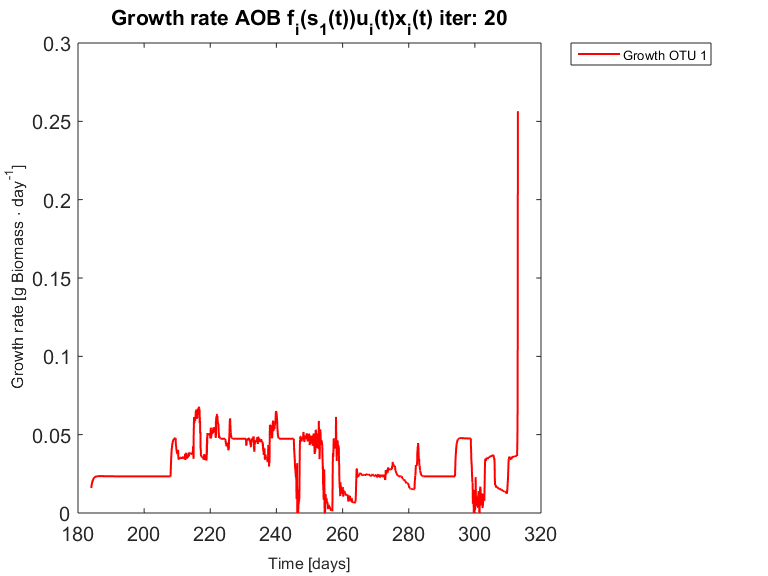
\includegraphics[width=\linewidth]{Application/200407_regroup_OTU_try2_iter_20_growth_control_AOB_plot_1}
		\caption{Growth rate of the model for AOB community.}
		\label{AOB_growth_control_application}
	\end{subfigure}
	\begin{subfigure}{0.45 \linewidth}
		\centering
		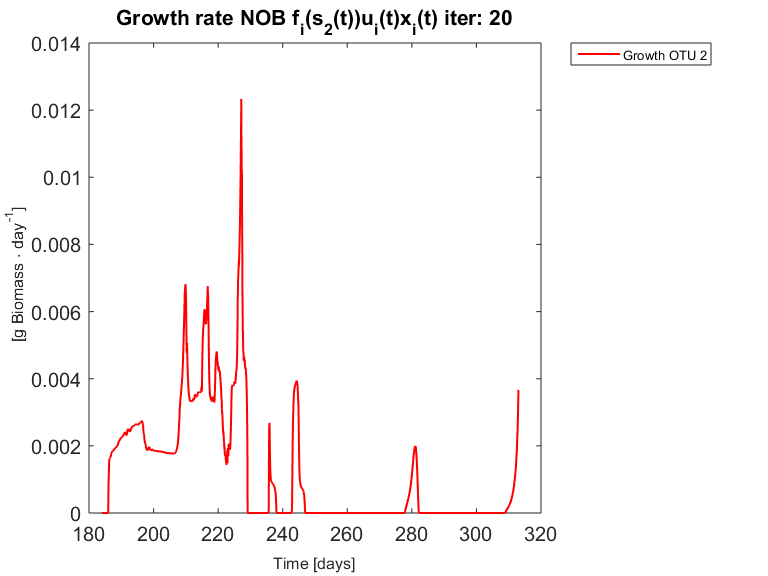
\includegraphics[width=\linewidth]{Application/200407_regroup_OTU_try2_iter_20_growth_control_NOB_plot_1}
		\caption{Growth rate of the model for the NOB community.}
		\label{NOB_growth_control_application}
	\end{subfigure}
	\caption{Obtained growth rates when regrouping OTU in their functional groups.}
	\label{growth_application}
\end{figure}



\begin{figure}[h]
	\centering
	\begin{subfigure}{0.45 \linewidth}
		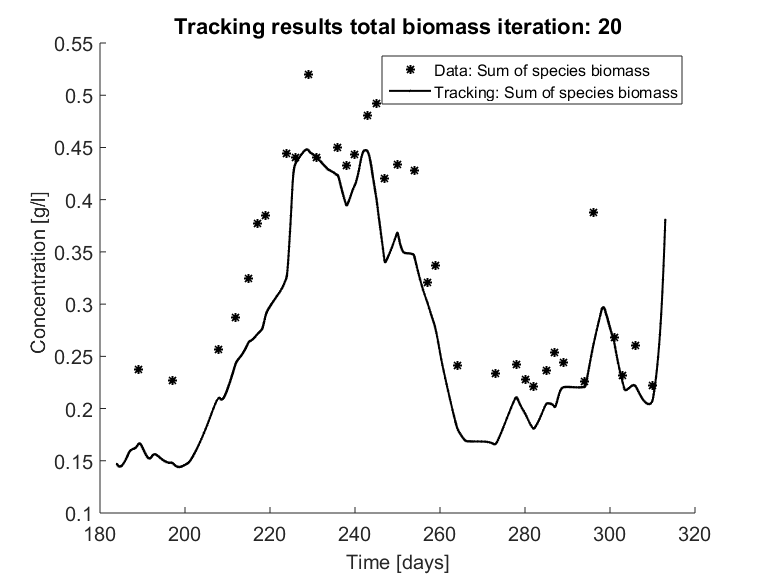
\includegraphics[width= \textwidth]{Application/200407_iter_20_Biomass}
		\caption{Total Biomass.}
		\label{Total Biomass application all}
	\end{subfigure}
	~
	\begin{subfigure}{0.45 \linewidth}
		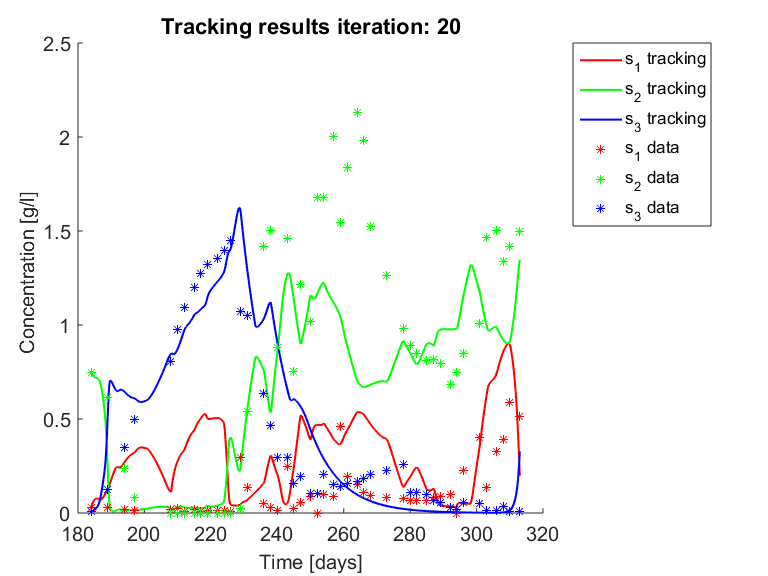
\includegraphics[width=\textwidth]{Application/200407_iter_20_metabolites}
		\caption{Metabolites.}
		\label{Metabolites application all}
	\end{subfigure}
	\caption{Results on applying the tracking method to a nitrification experiment when all OTU are tracked independently. Data points are represented by a star. The continuous line represents the tracking procedure results.}
	\label{all_OTU_results}
\end{figure}

\begin{figure}[h]
	\centering
	\begin{subfigure}{0.45 \textwidth}
		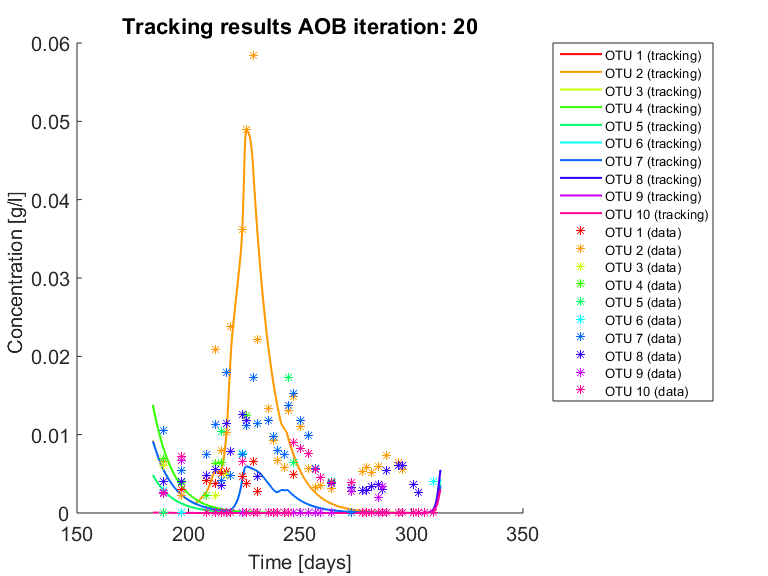
\includegraphics[width =\textwidth]{Application//200407_iter_20_AOB_plot_1}
	\end{subfigure}
	\begin{subfigure}{0.45 \textwidth}
	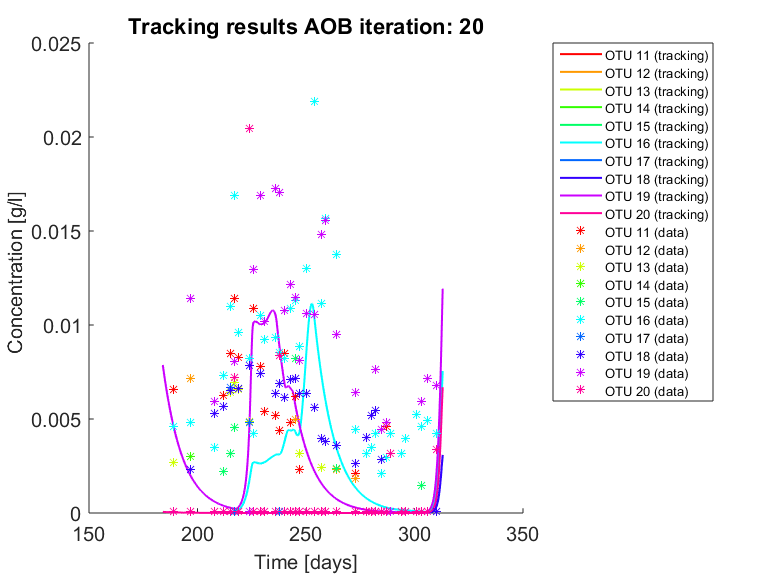
\includegraphics[width =\textwidth]{Application//200407_iter_20_AOB_plot_2}
	\end{subfigure}
	\begin{subfigure}{0.45 \textwidth}
	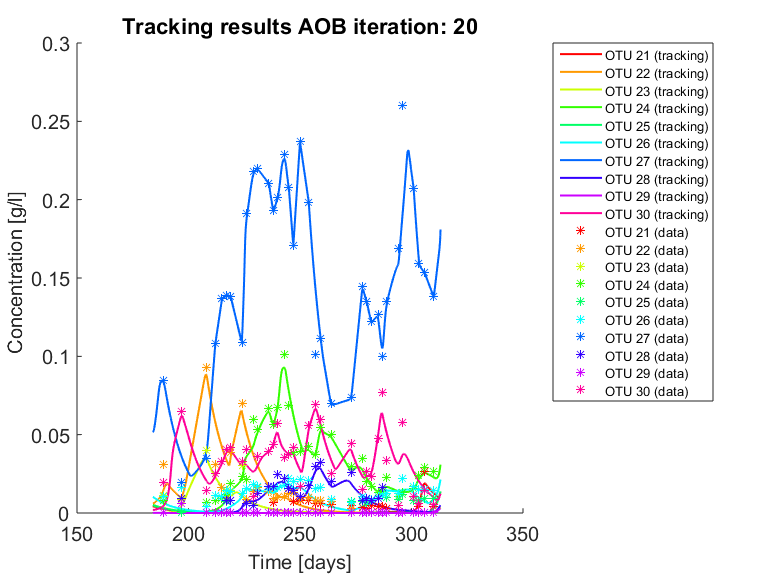
\includegraphics[width =\textwidth]{Application//200407_iter_20_AOB_plot_3}
	\end{subfigure}
	\begin{subfigure}{0.45 \textwidth}
	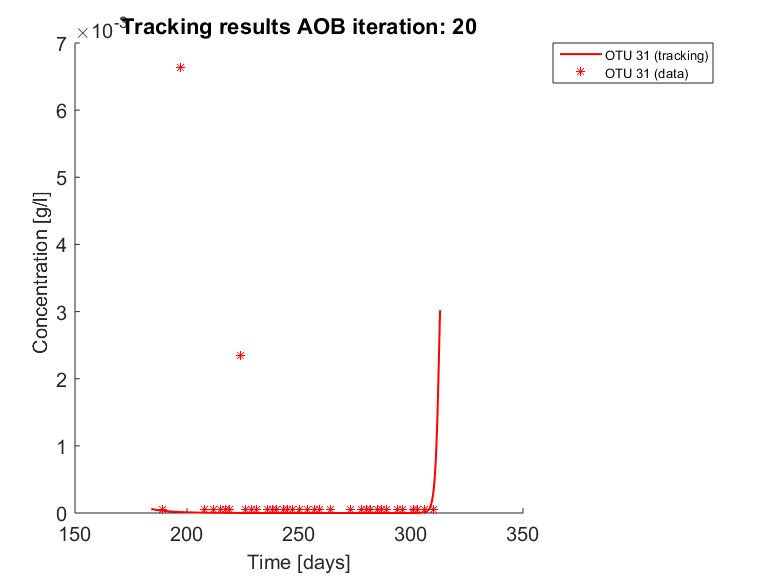
\includegraphics[width =\textwidth]{Application//200407_iter_20_AOB_plot_4}
	\end{subfigure}
	\begin{subfigure}{0.45 \textwidth}
	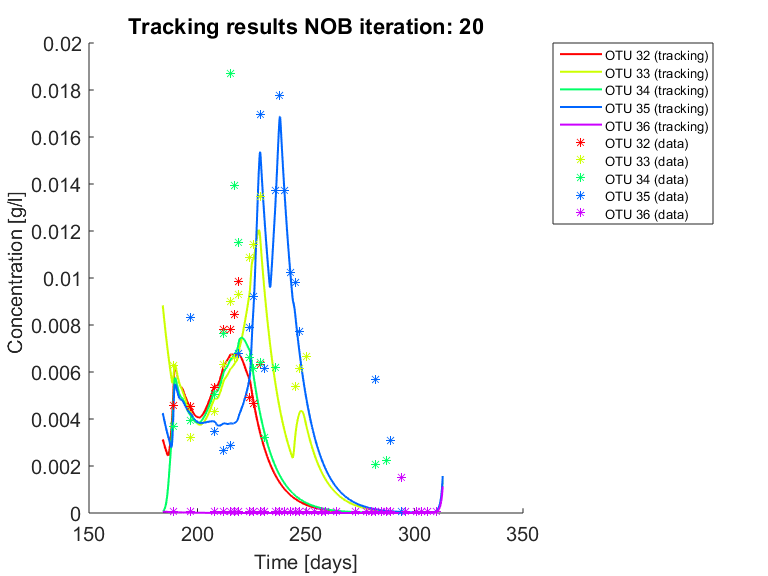
\includegraphics[width =\textwidth]{Application//200407_iter_20_NOB_plot_1}
	\end{subfigure}
	\caption{Tracking results when all OTU are tracked independently.}
	\label{OTU abudance all}
\end{figure}


\begin{figure}[h]
	\centering
	\begin{subfigure}{0.45 \textwidth}
		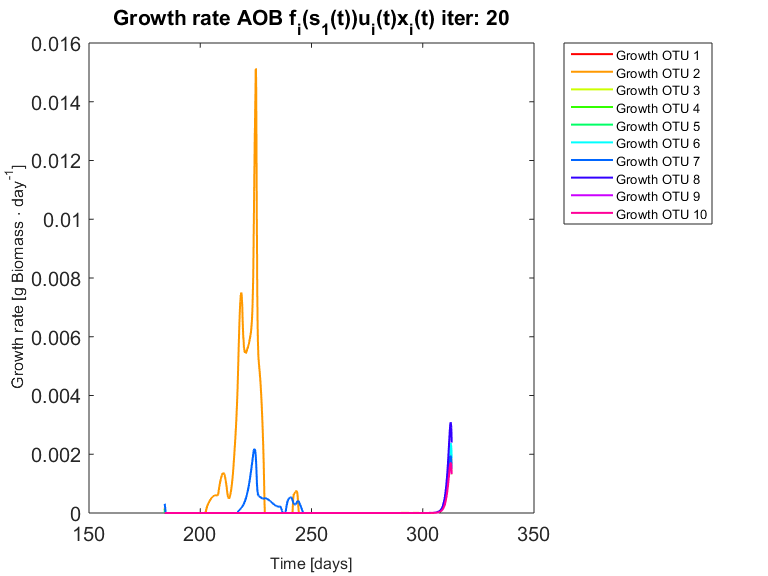
\includegraphics[width =\textwidth]{Application//200407_iter_20_growth_control_AOB_plot_1}
	\end{subfigure}
	\begin{subfigure}{0.45 \textwidth}
		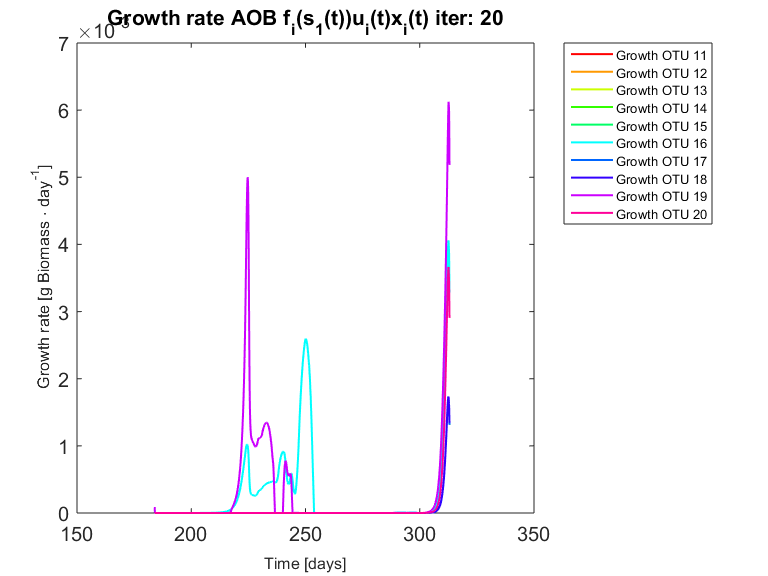
\includegraphics[width =\textwidth]{Application//200407_iter_20_growth_control_AOB_plot_2}
	\end{subfigure}
	\begin{subfigure}{0.45 \textwidth}
		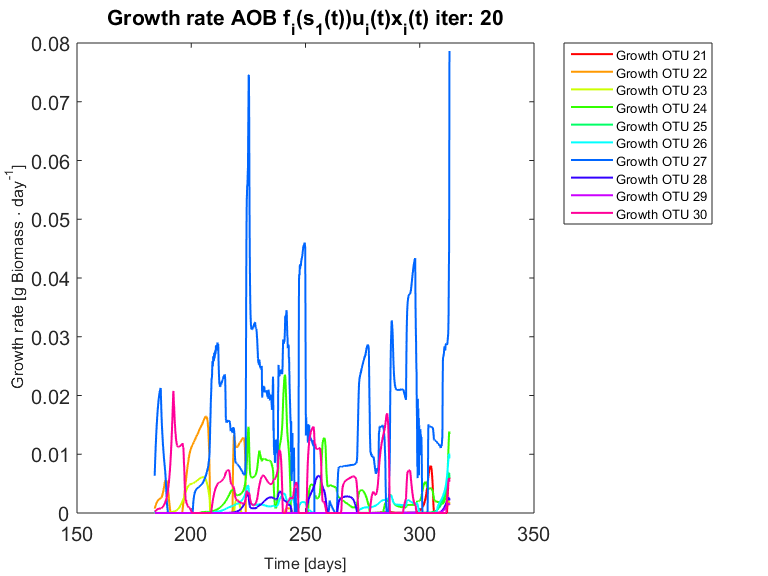
\includegraphics[width =\textwidth]{Application//200407_iter_20_growth_control_AOB_plot_3}
	\end{subfigure}
	\begin{subfigure}{0.45 \textwidth}
		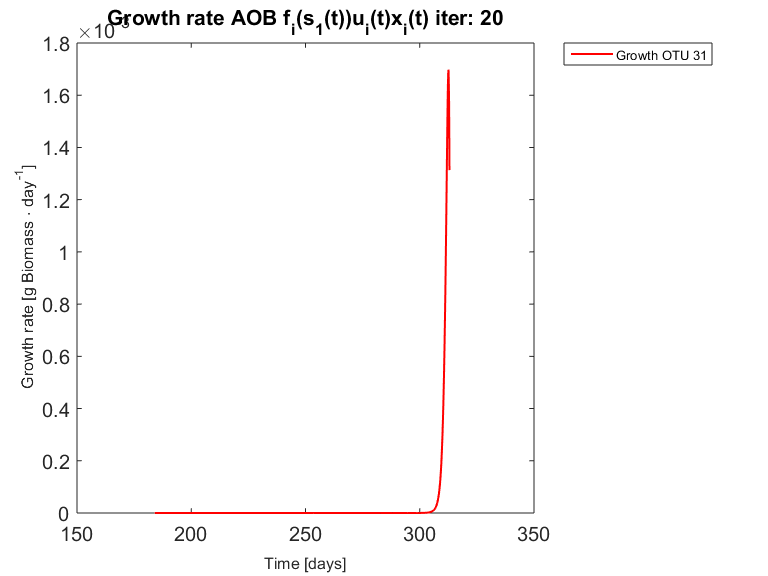
\includegraphics[width =\textwidth]{Application//200407_iter_20_growth_control_AOB_plot_4}
	\end{subfigure}
	\begin{subfigure}{0.45 \textwidth}
	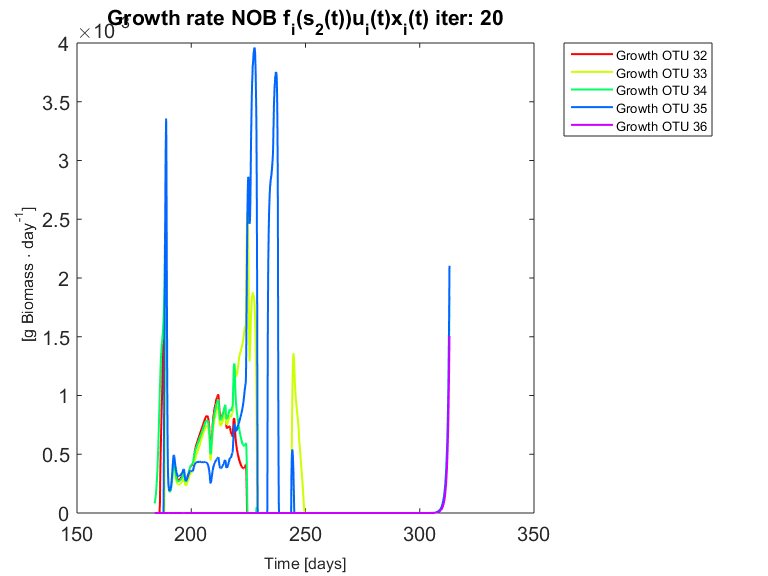
\includegraphics[width =\textwidth]{Application//200407_iter_20_growth_control_NOB_plot_1}
	\end{subfigure}
	\caption{Growth rates obtained for each OTU when applying the tracking procedure without aggregation.}
	\label{growth all}
\end{figure}


\clearpage
\section{Conclusions and Perspectives}

Last decades advances in genetic sequencing and microbial ecology has opened a gap for modellers in biochemical reactors to integrate this valuable information. Considering the success of mass balance models to predict and pilot bioreactors, one should build upon these existing models. This article proposed a naïve approach to start filling the gap of microbial ecology and biochemical process modelling: The approach can be simply described as correcting the growth rate of each individual species from genetic sequencing measurements, and observing what would that imply according to the (pseudo)stoichiometric equations involved. If one already posses a model for describing a particular bioprocess the use of the techniques here presented can be applied in a straightforward manner if one has already identified the microbial species involved with a particular functionality of the system.

The tracking model was proposed  in a chemostat setting as a way to correct a substrate limited expression. However the technique could be used in contexts where less information on the growth function of microbes is known. If one supposes nothing on the growth expression but the fact that is bounded (life cannot grow infinitely fast) the model becomes a linear model and one recovers a classic quadratic regulator for linear systems. Nevertheless, even in the former case, the synthesis of the optimal bounded control remains an open theoretical challenge.

The interaction function introduced tries to address the issue of prediction from genetic sequencing. The analysis of the gLV model proposed by Dumont \textit{et al.} \cite{Dumont2016} shows that such a model structure can give way to bi-stability, coexistence within a functional group, and unintuitive operational insights such as raising the input ammonium $s_{in}$ to achieve partial nitrification. From the application section one can see that by correcting the growth rate one is able to recuperate the substrates dynamics, suggesting that interactions are driving the system. This opens the question for a broader class of interaction functions that could represent well complex microbial ecosystems, particularly biorreactors. 

One of the next steps in this line of research would be to synthesize a control that is able to reconstruct the interaction functions, and not just the dynamics of the species. One might bypass the end point issue of the current control scheme by, for example, by a very thorough use of the pontryagin maximum principle for the synthesis of the control. In a more general view the reconstruction of the growth function in chemostat systems is already subject to problems of identifiability: integrating genetic sequencing could provide a path for more certainty in model calibration.




\section{Codes}

All the codes can be recovered from the following repository \url{https://github.com/paus-5/Class-and-Track}.
\section{Acknowledgements}
 The authors would like to thank Alain Rapaport for the fruitful exchanges. This work was financed by project Thermomic ANR-16-CE04-0003.

\section{Supplementary Material}


\textbf{Proof of lemma \ref{l1}}
\begin{proof}
	Define 
	\begin{align}
	z_1 &: = \sum \limits_{i \in G_1} \frac{1}{y_i}x_i + s_1  \\
	z_2 &: = \sum \limits_{i \in G_2} \frac{1}{y_i}x_i + s_1 + s_2 \\
	z_3 &: = s_1 + s_2 + s_3
	\end{align} 
	
	Computing $\dot{z_{1}}$ one gets:
	\begin{align*}
	\dot{z_{1}} &=\sum \limits_{i \in G_1} \frac{1}{y_i}\dot{x_i} + \dot{s_1} \\
	& = \sum \limits_{i \in G_1} \frac{1}{y_i}\left(\mu_i(s_1,x) -D \right)x_i + (s_{in}-s_1)D-\sum\limits_{i \in G_1}\frac{1}{y_i}\mu_i(s_1,x) x_i   \\
	&= 	D\left(-\sum \limits_{i \in G_1} \frac{1}{y_i}x_i - s_1 + s_{in}\right)  \\
	& = D(s_{in} - z_1)
	\end{align*}
	
	Define $\bar{s} =\max\{s_{in}(t) | t\geq 0\}$ and consider the differential equation:
	
	\begin{align}
	\label{compareEquation}
	\begin{array}{l}
	\dot{w} = D(\bar{s} - w) \\
	w(0) = \sum \limits_{i \in G_1} \frac{1}{y_i}x_i(0) + s_1(0)
	\end{array}
	\end{align}
	
	If there is a time interval $H$ such that $t^*\in H  \Rightarrow D(t^*) = 0$, then $z_1$ is constant and therefore bounded by  the value of the solution in $z(t^*)$. 
	If $D(t) > 0$, then $w = \bar{s}$ is a stable asymptotic equilibrium. Define $M_1 :=  \max\{w(0),\bar{s}\}$. If $ w(0) > \bar{s}$ then by the Picard-Lindeloff theorem $ \forall t \; \dot{w}(t) < 0 $, otherwise it would cross the solution of the initial value problem \eqref{compareEquation} with starting point $\bar{s}$ , therefore $w(t) \geq \bar{s}$. The same reasoning may be applied if $ w(0) < \bar{s}$. One concludes that $ w(t) \leq M_1 $. 
	
	Consider  
	\begin{align}
	\label{z1} \begin{array}{l}
	\dot{z_1} =  D(s_{in} - z_1)\\
	z_1(0) = \sum \limits_{i \in G_1} \frac{1}{y_i}x_i(0) + s_1(0)
	\end{array} 
	\end{align}
	From a comparison lemma (see chapter 3 \cite{Khalil1996}), the solution of \eqref{z1} is bounded by $w$ and therefore $z_1(t) \leq M_1$.
	
	By defining $M_2 = \max\left \{ \displaystyle \sum \limits_{i=n_1 +1 }^{n} \frac{1}{y_i}x_i(0) + s_1(0) +s_2(0), \bar{s} \right\}$, and $M_3 =\max\left \{ s_1(0) +s_2(0) + s_3(0), \bar{s} \right\} $ and noting that $z_2(t)$ and $z_3(t)$ satisfies the same differential equations as $z_1$ the above reasoning may be applied and one has the desired bounds.
\end{proof}

\textbf{Proof of theorem \ref{theoWellPosedness}}

\begin{proof}
	If any coordinate of the solution becomes zero, then it's derivative is either zero, or positive. The bound will follow from Lemma \ref{l1}.
	
	Note that for any $i \in \{1,\dots, n\} $ if $x_i = 0$ then $\dot{x_{i}} = 0$, therefore all solutions of system \eqref{system} with initial condition $x_i(t_0) = 0$ remain in these planes. By the Picard Lindeloff theorem a solution starting in $int(\Omega)$ cannot cross these planes, therefore $x_i(t)\geq 0$ for $t \geq 0$.
	
	If $s_1 = 0$, then $\dot{s_1} = Ds_{in} > 0$. Therefore $s_1(t) \geq 0$.
	
	If $s_2 = 0$ then note first that by adding both inequalities from Lemma \eqref{l1} and since, $s_1,x_i \geq 0$ one has:
	\begin{align*}
	\sum \limits_{i \in G_1 \cup G_2}  \frac{1}{y_i} x_i + 2s_1 + s_2 \leq M_1 + M_2 \\
	\Rightarrow \sum \limits_{i = 1}^{n}  \frac{1}{y_i} x_i + 2s_1 \leq M_1 + M_2 \\
	\Rightarrow \sum \limits_{i = 1}^{n}  \frac{1}{y_i} x_i \leq M_1 + M_2\\ 
	\Rightarrow \bar{k} \sum  \limits_{i = 1}^{n}   x_i  \leq M_1 + M_2  \\
	\Leftrightarrow \bar{k} \sum  \limits_{i = 1}^{n}   \vert x_i \vert  \leq M_1 + M_2  \\
	\Leftrightarrow \bar{k} \Vert x \Vert_1  \leq M_1 + M_2  \\
	\Rightarrow   \bar{k} \Vert x \Vert_{\infty} \leq M_1 + M_2
	\end{align*}
	
	Where $\bar{k} = \min \left\{ \frac{1}{y_i}  : \; i\in [n] \right \}$.
	
	Define $M := \dfrac{\bar{k}}{M_1 + M_2}$, and let $A$ be a matrix such that $\Vert A \Vert_{\infty} \leq M$. Then since $\Vert Ax \Vert_{\infty} \leq 1 \Rightarrow \forall i=1,\dots,n \; (1 + A_{i\bullet}x) \geq 0 $, and $\Vert Ax \Vert_{\infty} \leq \Vert A \Vert_{\infty} \Vert x\Vert_{\infty} \leq M \frac{1}{M}$.
	One has proven that:
	\begin{align}
	\label{Bound1} \forall i=1,\dots,n \;  \;  (1 + A_{i\bullet}x) \geq 0 
	\end{align} 
	
	Therefore $\dot{s_2} = \displaystyle \sum \limits_{i \in G_1 } \frac{1}{y_i}\mu_i(s_1,x)x_i =  \sum \limits_{i \in G_1 } \frac{1}{y_i}\bar{\mu_i}f_i(s)(1+A_{i \bullet }x)x_i \geq 0$. Therefore $s_2(t) \geq 0$.
	
	Note that since one has proven that $s_2 \geq 0$, bound \eqref{Bound1} is valid for any time, and not only when $s_2 = 0$. 
	If $s_3 = 0$ then $\dot{s_3} = \sum \limits_{i \in G_2 }^{n}\frac{1}{y_i}\mu_i(s_2,x)\geq 0$. Therefore $s_3 \geq 0$.
	
	For the boundedness it suffices to notice from Lemma \ref{l1} that the sum of positive elements is bounded, therefore each element is bounded.
\end{proof}

\subsection{Properties of diag operator}

Notice that for two vectors $v_1$ and $v_2$ the following holds:
\begin{align}
\diag(v_1)\diag(v_2) = \diag(v_2)\diag(v_1) 
\end{align}

Suppose $v \in \R^n$ such that $v_i \neq 0 \forall i \in [n]$. Define $v^{-1}:= \left( \dfrac{1}{v_1},\dots,\dfrac{1}{v_n} \right)$ then the inverse of $\diag(v)$ exists and is $\diag(v^{-1})$:

\begin{align}
\diag(v)^{-1} = \diag(v^{-1}) 
\end{align}

\subsection{Inverse of A and products}
Notice that $\begin{bmatrix}
A_1 \\ A_2
\end{bmatrix} A^{-1} = \begin{bmatrix}
A_1A^{-1} \\ A_2A^{-1}
\end{bmatrix}=I $.

Then $A_1A^{-1}= \begin{bmatrix}
I_{n_1}& 0_{n_2 \times 1} 
\end{bmatrix}$ and $A_2A^{-1}= \begin{bmatrix}
0_{n_1 \times 1} & I_{n_2}
\end{bmatrix}$.

For notation purposes it is useful to define: \begin{align}
B := \diag(k) A^{-1}.
\end{align}

\subsection{Deduction of  \eqref{s1Equilibria}}

Replacing \eqref{xEquilibria} in \eqref{Eq2} yields :
\begin{align}
(s_{in}-s_1)D- \begin{bmatrix}
1_{n_1 \times 1}+A_1A^{-1}(\diag(f(s))^{-1}D_{n_1 \times 1}-1_{n_1 \times 1}) \\0_{n_2 \times 1}
\end{bmatrix}^\top \diag(k)\diag(f(s))A^{-1}(\diag(f(s))^{-1}D_{n \times 1}-1_{n \times 1})=0 \\
(s_{in}-s_1)D-	\begin{bmatrix}
1_{n_1 \times 1}+\begin{bmatrix}
I_{n_1} & 0_{n_2 \times 1} 
\end{bmatrix}(\diag(f(s))^{-1}D_{n \times 1}-1_{n \times 1}) \\0_{n_2\times 1}
\end{bmatrix}^\top \diag(k)\diag(f(s))A^{-1}(\diag(f(s))^{-1}D_{n \times 1}-1_{n \times 1}) = 0 \\
(s_{in}-s_1)D-	\begin{bmatrix}
D_{n_1 \times 1}\\0_{n_2 \times 1}
\end{bmatrix}^T\diag(f(s))^{-1}\diag(f(s)) \diag(k) A^{-1}(\diag(f(s))^{-1}D_{n \times 1}-1_{n \times 1}) = 0  \\
(s_{in}-s_1)D-\begin{bmatrix}
D_{n_1 \times 1} \\0_{n_2\times 1}
\end{bmatrix}^\top \diag(k)A^{-1}(\diag(f(s))^{-1}D_{n \times 1}-1_{n_1 \times 1}) = 0 \\
(s_{in}-s_1)- \begin{bmatrix}
1_{n_1 \times 1}\\0_{n_2 \times 1}
\end{bmatrix}^\top B (\diag(f(s))^{-1}D_{n \times 1} - 1_{n \times 1}) = 0 
\end{align}

\subsection{Deduction of \eqref{s2Equilibria}}
Analogous as before, replacing \eqref{xEquilibria} in \eqref{Eq3} yields :
\begin{align}
-s_2D+
\begin{bmatrix}
(\diag(\mu_A)^{-1} \vec{D}) \\ -(\diag(\mu_B)^{-1} \vec{D})
\end{bmatrix}^\top \diag(\mu)\diag(y)^{-1} A^{-1}(\diag(\mu)^{-1}\vec{D}-\vec{1}) = 0 \\
-s_2D+
\begin{bmatrix}
\vec{D} \\ - \vec{D}
\end{bmatrix}^\top \diag(y)^{-1} A^{-1}(\diag(\mu)^{-1}\vec{D}-\vec{1}) = 0\\
-s_2+
\begin{bmatrix}
\vec{1} \\ - \vec{1}
\end{bmatrix}^\top B(\diag(\mu)^{-1}\vec{D}-\vec{1}) = 0
\end{align}
\begin{align} 
-s_2D+ \begin{bmatrix}
1_{n_1 \times 1}+A_1A^{-1}(\diag(f(s))^{-1}D_{n_1 \times 1}-1_{n_1 \times 1}) \\-(1_{n_1 \times 1}+A_2A^{-1}(\diag(f(s))^{-1}D_{n_1 \times 1}-1_{n_1 \times 1})
\end{bmatrix}^\top \diag(k)\diag(f(s))A^{-1}(\diag(f(s))^{-1}D_{n \times 1}-1_{n \times 1}) = 0 \\
-s_2D+	\begin{bmatrix}
1_{n_1 \times 1}+\begin{bmatrix}
I_{n_1} & 0_{n_2 \times 1} 
\end{bmatrix}(\diag(f(s))^{-1}D_{n \times 1}-1_{n \times 1}) \\-(1_{n_1 \times 1}+\begin{bmatrix}
0_{n_1 \times 1} & I_{n_2} 
\end{bmatrix}(\diag(f(s))^{-1}D_{n_1 \times 1}-1_{n_1 \times 1})
\end{bmatrix}^\top \diag(k)\diag(f(s))A^{-1}(\diag(f(s))^{-1}D_{n \times 1}-1_{n \times 1}) = 0 \\
-s_2D +	\begin{bmatrix}
D_{n_1 \times 1}\\-D_{n_2 \times 1}
\end{bmatrix}^T\diag(f(s))^{-1}\diag(f(s)) \diag(k) A^{-1}(\diag(f(s))^{-1}D_{n \times 1}-1_{n \times 1}) = 0  \\
-s_2D+\begin{bmatrix}
D_{n_1 \times 1} \\-D_{n_2\times 1}
\end{bmatrix}^\top \diag(k)A^{-1}(\diag(f(s))^{-1}D_{n \times 1}-1_{n_1 \times 1}) = 0 \\
-s_2 + \begin{bmatrix}
1_{n_1 \times 1}\\1_{n_2 \times 1}
\end{bmatrix}^\top B (\diag(f(s))^{-1}D_{n \times 1} - 1_{n \times 1}) = 0 
\end{align}
\subsection{Deduction of \eqref{S2(S1)}}


Note that 
\begin{align}  (\diag(f(s))^{-1}D_{n\times 1}-1_{n\times1})  & = \begin{array}{cc} 
\begin{bmatrix}
\left(D\frac{K_1+s_1}{\bar{\mu}_{1}s_1}-1 \right) \\ \vdots \\ \left(D\frac{K_n+s_2}{\bar{\mu}_{n}s_2}-1\right) 
\end{bmatrix} & \hspace{-0.5cm}\begin{array}{c} \left\} n_1\right. \\ \\ \left\} n_2\right.\end{array}
\end{array} \\
\label{invMu} 
& = \begin{bmatrix}
\dfrac{DK_1+(D-\bar{\mu}_1)s_1}{\bar{\mu}_{1}s_1} \\ \vdots \\ \dfrac{DK_n+(D-\bar{\mu}_n)s_2}{\bar{\mu}_{n}s_2} 
\end{bmatrix}
\end{align}

Replacing \eqref{invMu} in \eqref{s1Equilibria}.

\begin{align}
(s_{in}-s_1)-	\begin{bmatrix}
1_{n_1 \times 1} \\0_{n_2\times 1}
\end{bmatrix}^\top  B\begin{bmatrix}
\dfrac{DK_1+(D-\bar{\mu}_1)s_1}{\bar{\mu}_{1}s_1} \\ \vdots \\ \dfrac{DK_n+(D-\bar{\mu}_n)s_2}{\bar{\mu}_{n}s_2} 
\end{bmatrix} = 0 \\
(s_{in}-s_1) - \sum \limits_{i=1}^{n_1}\left(\sum \limits_{j = 1}^{n_1} B_{ij}\dfrac{DK_j+(D-\bar{\mu}_j)s_1}{\bar{\mu}_{j}s_1} +\sum \limits_{j = n_1+1}^{n} B_{ij}\dfrac{DK_j+(D-\bar{\mu}_j)s_2}{\bar{\mu}_{j}s_2} \right) = 0 \quad / \cdot s_1s_2 \\
(s_{in}-s_1)s_1s_2 - \sum \limits_{i=1}^{n_1}\left(\sum \limits_{j = 1}^{n_1} B_{ij}\dfrac{DK_j+(D-\bar{\mu}_j)s_1}{\bar{\mu}_{j}}s_2 +\sum \limits_{j = n_1+1}^{n} B_{ij}\dfrac{DK_j+(D-\bar{\mu}_j)s_2}{\bar{\mu}_{j}}s_1 \right) = 0 \\
(s_{in}-s_1)s_1s_2 - \sum \limits_{i=1}^{n_1}\left(\sum \limits_{j = 1}^{n_1} B_{ij}\dfrac{DK_j}{\bar{\mu}_{j}}s_2 +\sum \limits_{j = 1}^{n} B_{ij}\dfrac{(D-\bar{\mu}_j)}{\bar{\mu}_{j}}s_2s_1 + \sum \limits_{j = n_1+1}^{n} B_{ij}\dfrac{DK_j}{\bar{\mu}_{j}}s_1 \right) = 0  \\
s_2\left((s_{in}-s_1)s_1 - \sum \limits_{i=1}^{n_1}  \left( \sum \limits_{j = 1}^{n_1} B_{ij}\dfrac{DK_j}{\bar{\mu}_{j}} + \sum \limits_{j = 1}^{n} B_{ij}\dfrac{(D-\bar{\mu}_j)}{\bar{\mu}_{j}}s_1 \right)  \right) =  \sum \limits_{i=1}^{n_1}\sum \limits_{j = n_1+1}^{n} B_{ij}\dfrac{DK_j}{\bar{\mu}_{j}}s_1 \\
s_2\left(-s_{1}^2  +  \left( s_{in}\underbrace{- \sum \limits_{i=1}^{n_1} \sum \limits_{j = 1}^{n} B_{ij}\dfrac{(D-\bar{\mu}_j)}{\bar{\mu}_{j}}}_{\beta_1}\right) s_1 \underbrace{ - \sum \limits_{i=1}^{n_1}  \sum \limits_{j = 1}^{n_1} B_{ij}\dfrac{DK_j}{\bar{\mu}_{j}}}_{\beta_2}  \right) = \underbrace{\sum \limits_{i=1}^{n_1}\sum \limits_{j = n_1+1}^{n} B_{ij}\dfrac{DK_j}{\bar{\mu}_{j}}}_{\beta_3}s_1 \\
s_2\left(-s_{1}^2  +  \left( s_{in}+\beta_1 \right) s_1 +\beta_2  \right) = \beta_3 s_1
\end{align} 

From the last expression it should be clear that formula \eqref{S2(S1)} holds, it is just a matter of identifying the coefficients.
\begin{itemize}
	\item $\beta_1 =  - \sum \limits_{i=1}^{n_1} \sum \limits_{j = 1}^{n} B_{ij}\dfrac{(D-\bar{\mu}_j)}{\bar{\mu}_{j}}$
	\item $\beta_2 =-\sum \limits_{i=1}^{n_1}  \sum \limits_{j = 1}^{n_1} B_{ij}\dfrac{DK_j}{\bar{\mu}_{j}}$
	\item $\beta_3 = \sum \limits_{i=1}^{n_1}\sum \limits_{j = n_1+1}^{n} B_{ij}\dfrac{DK_j}{\bar{\mu}_{j}} $
	\item $c_1 = \dfrac{-1}{\beta_3}$
	\item $c_2 =  \dfrac{s_{in} + \beta_1}{\beta_3}$
	\item $c_3 = \dfrac{\beta_2}{\beta_3}$
\end{itemize}

\subsection{Deduction of \eqref{Poly4}}

Again, replacing \eqref{invMu} in \eqref{s2Equilibria}.
\begin{align}
-s_2+
\begin{bmatrix}
1_{n_1 \times 1}\\ - 1_{n_2 \times 1}
\end{bmatrix}^\top B\begin{bmatrix}
\dfrac{DK_1+(D-\bar{\mu}_1)s_1}{\bar{\mu}_{1}s_1} \\ \vdots \\ \dfrac{DK_n+(D-\bar{\mu}_n)s_2}{\bar{\mu}_{n}s_2} 
\end{bmatrix} = 0 \\
\begin{array}{c} \displaystyle  -s_2 + \sum \limits_{i=1}^{n_1}\left(\sum \limits_{j = 1}^{n_1} B_{ij}\dfrac{DK_j+(D-\bar{\mu}_j)s_1}{\bar{\mu}_{j}s_1} +\sum \limits_{j = n_1+1}^{n} B_{ij}\dfrac{DK_j+(D-\bar{\mu}_j)s_2}{\bar{\mu}_{j}s_2} \right) \\
\displaystyle - \sum \limits_{i=n_1+1}^{n}\left(\sum \limits_{j = 1}^{n_1} B_{ij}\dfrac{DK_j+(D-\bar{\mu}_j)s_1}{\bar{\mu}_{j}s_1} +\sum \limits_{j = n_1+1}^{n} B_{ij}\dfrac{DK_j+(D-\bar{\mu}_j)s_2}{\bar{\mu}_{j}s_2} \right)= 0
\end{array} \quad / \cdot s_1s_2 \\
\begin{array}{c} \displaystyle  -s_1s_2^2 +\sum \limits_{i=1}^{n_1}\left(\sum \limits_{j = 1}^{n_1} B_{ij}\dfrac{DK_j+(D-\bar{\mu}_j)s_1}{\bar{\mu}_{j}}s_2 +\sum \limits_{j = n_1+1}^{n} B_{ij}\dfrac{DK_j+(D-\bar{\mu}_j)s_2}{\bar{\mu}_{j}}s_1 \right) \\
\displaystyle -  \sum \limits_{i=n_1+1}^{n}\left(\sum \limits_{j = 1}^{n_1} B_{ij}\dfrac{DK_j+(D-\bar{\mu}_j)s_1}{\bar{\mu}_{j}}s_2 +\sum \limits_{j = n_1+1}^{n} B_{ij}\dfrac{DK_j+(D-\bar{\mu}_j)s_2}{\bar{\mu}_{j}}s_1 \right)= 0
\end{array} \\
\begin{array}{c} \displaystyle  -s_1s_2^2 + \sum \limits_{i=1}^{n_1}\left(\sum \limits_{j = 1}^{n_1} B_{ij}\dfrac{DK_j}{\bar{\mu}_{j}}s_2 +\sum \limits_{j = 1}^{n} B_{ij}\dfrac{(D-\bar{\mu}_j)}{\bar{\mu}_{j}}s_2s_1 + \sum \limits_{j = n_1+1}^{n} B_{ij}\dfrac{DK_j}{\bar{\mu}_{j}}s_1\right) \\
\displaystyle -  \sum \limits_{i=n_1+1}^{n}\left(\sum \limits_{j = 1}^{n_1} B_{ij}\dfrac{DK_j}{\bar{\mu}_{j}}s_2 +\sum \limits_{j = 1}^{n} B_{ij}\dfrac{(D-\bar{\mu}_j)}{\bar{\mu}_{j}}s_2s_1 + \sum \limits_{j = n_1+1}^{n} B_{ij}\dfrac{DK_j}{\bar{\mu}_{j}}s_1 \right)= 0
\end{array}\\
\begin{array}{c} \displaystyle  -s_1s_2^2  - \beta_2s_2 -\beta_1s_1s_2 + \beta_3s_1 
\underbrace{- \sum \limits_{i=n_1+1}^{n}\sum \limits_{j = 1}^{n_1} B_{ij}\dfrac{DK_j}{\bar{\mu}_{j}}}_{\beta_4}s_2 \underbrace{-\sum \limits_{i=n_1+1}^{n}\sum \limits_{j = 1}^{n} B_{ij}\dfrac{(D-\bar{\mu}_j)}{\bar{\mu}_{j}}}_{\beta_5}s_2s_1\underbrace{ -\sum \limits_{i=n_1+1}^{n}\sum \limits_{j = n_1+1}^{n} B_{ij}\dfrac{DK_j}{\bar{\mu}_{j}}}_{\beta_6}s_1 = 0
\end{array}\\
-s_1s_2^2  - \beta_2s_2 -\beta_1s_1s_2 + \beta_3s_1 + \beta_4s_2 +\beta_5s_1s_2 + \beta_6s_1  = 0 \\
\label{Prepoly4} (\beta_4-\beta_2)s_2 + (\beta_3+\beta_6)s_1 + (\beta_5 - \beta_1)s_1s_2- s_1s_2^2 = 0 
\end{align}
\begin{itemize}
	\item  $\displaystyle  \beta_4 = - \sum \limits_{i=n_1+1}^{n}\sum \limits_{j = 1}^{n_1} B_{ij}\dfrac{DK_j}{\bar{\mu}_{j}}$
	\item $\displaystyle  \beta_5 = -\sum \limits_{i=n_1+1}^{n}\sum \limits_{j = 1}^{n} B_{ij}\dfrac{(D-\bar{\mu}_j)}{\bar{\mu}_{j}}$
	\item $\displaystyle \beta_6 =  -\sum \limits_{i=n_1+1}^{n}\sum \limits_{j = n_1+1}^{n} B_{ij}\dfrac{DK_j}{\bar{\mu}_{j}}$
\end{itemize}

Then replace \eqref{S2(S1)} in \eqref{Prepoly4}: 
\begin{align}
(\beta_4-\beta_2)\dfrac{s_1}{c_1s_1^2+c_2s_1+c_3} + (\beta_3+\beta_6)s_1 + (\beta_5 - \beta_1)s_1\dfrac{s_1}{c_1s_1^2+c_2s_1+c_3}- s_1\left(\frac{s_1}{c_1s_1^2+c_2s_1+c_3}\right)^2 = 0 \quad / \cdot \frac{1}{s_1} \\
(\beta_4-\beta_2)\dfrac{1}{c_1s_1^2+c_2s_1+c_3} + (\beta_3+\beta_6) + (\beta_5 - \beta_1)\dfrac{s_1}{c_1s_1^2+c_2s_1+c_3}- \left(\frac{s_1}{c_1s_1^2+c_2s_1+c_3}\right)^2 = 0  \quad / \cdot (c_1s_1^2+c_2s_1+c_3)^2 \\
(\beta_4-\beta_2)(c_1s_1^2+c_2s_1+c_3)+ (\beta_3+\beta_6)(c_1s_1^2+c_2s_1+c_3)^2 + (\beta_5 - \beta_1)(c_1s_1^2+c_2s_1+c_3)s_1 - s_1^2 = 0   \\
\begin{array}{c}(\beta_4-\beta_2)(c_1s_1^2+c_2s_1+c_3)+ (\beta_3+\beta_6)(c_1^2s_1^4+c_2^2s_1^2+c_3^2 + 2 c_1c_2s_1^3 + 2c_2c_3s_1 + 2 c_1c_3s_1^2)\\ \\  + (\beta_5 - \beta_1)(c_1s_1^2+c_2s_1+c_3)s_1 - s_1^2 = 0 \end{array} \\
\begin{array}{c} \underbrace{(\beta_3+\beta_6)c_1^2}_{a_4} s_1^4 + (\underbrace{(\beta_3 + \beta_6)(2c_1c_2) +  (\beta_5 -\beta_1)c_1}_{a_3})s_1^3 + (\underbrace{(\beta_4 - \beta_2)c_1 +(\beta_3 + \beta_6)(c_2^2 + 2c_1c_3) + (\beta_5-\beta_1)c_2-1}_{a_2})s_1^2 \\ 
+(\underbrace{(\beta_4 -\beta_2)c_2 + (\beta_3 + \beta_6)2c_2c_3+(\beta_5-\beta_1)c_3}_{a_1})s_1 + \underbrace{(\beta_4-\beta_2)c_3 + (\beta_3 + \beta_6)c_3^2}_{a_0} = 0
\end{array}
\end{align}

Which yields \eqref{Poly4}.
\begin{itemize}
	\item $a_4 = (\beta_3+\beta_6)c_1^2$ 
	\item $a_3 = (\beta_3 + \beta_6)(2c_1c_2) +  (\beta_5 -\beta_1)c_1$
	\item $a_2 = (\beta_4 - \beta_2)c_1 +(\beta_3 + \beta_6)(c_2^2 + 2c_1c_3) + (\beta_5-\beta_1)c_2-1$
	\item $a_1 = (\beta_4 -\beta_2)c_2 + (\beta_3 + \beta_6)2c_2c_3+(\beta_5-\beta_1)c_3$
	\item $a_0 = (\beta_4-\beta_2)c_3 + (\beta_3 + \beta_6)c_3^2$
\end{itemize}

\textbf{Note:} When calculating the equilibria with the extinction of some OTU under H \ref{noWashoutHyp}, coefficients are calculated with $B = \diag(k^{act})(A^{act})^{-1}$. The indexes are redefined to be taken only in $i,j \in [n] \setminus \mathcal{J}$ by formula \eqref{EquilibriaFormula}.

\subsection{Deduction of \eqref{S1NOBWashout}}
For auxiliary purposes $B:= \diag(k^{act})(A^{act})^{-1}$. 

Under hypothesis \ref{WashoutG2}, the $j \in \mathcal{J}$ entries of vector $\diag(k) \diag(f(s))x^{eq} $ are zero. 
Note also that $(A_1x^{eq})_i = (A^{act}x^{act})_i, \, \forall i \in [n] \setminus \mathcal{J}$.

Then the cross product in equation \eqref{Eq2} can be reduced:
\begin{align} 
\begin{bmatrix}
1_{n_1\times 1}+A_1x^{eq} \\0
\end{bmatrix}^\top \diag(k) \diag(f(s))x^{eq} = [1_{(n-m)\times 1} - A^{act}x^{act}]^\top \diag(k^{act}) \diag(f^{act}(s))x^{act} 
\end{align} 
Therefore replacing \eqref{EquilibriaFormula} and \eqref{EqSome} in \eqref{Eq2}.

\begin{align}
0 &= (s_{in}-s_1)D- [1_{(n-m)\times 1} - A^{act}x^{act}]^\top \diag(k^{act}) \diag(f^{act}(s))x^{act}\\
&= (s_{in}-s_1)D- [1_{(n-m)\times 1} - A^{act}(A^{act})^{-1}(\diag(f^{act}(s))^{-1}D_{(n-m)\times 1} - 1_{(n-m)\times 1})]^\top \dots \\ & \diag(k^{act}) \diag(f^{act}(s))(A^{act})^{-1}(\diag(f^{act}(s))^{-1}D_{(n-m)\times 1} - 1_{(n-m)\times 1})\\
&  =  (s_{in}-s_1)-1_{(n-m)\times 1}^\top
B(\diag(f^{act}(s))^{-1}D_{(n-m)\times 1} - 1_{(n-m)\times 1})
\end{align} 


$s_2$ does not appear in the previous equation. Then as before (using the numeration of active indexes):
\begin{align}
\diag(\mu^{act})^{-1}D_{(n-m)\times 1} - 1_{(n-m)\times 1} = \begin{bmatrix}
\dfrac{DK_1+(D-\bar{\mu}_1)s_1}{\bar{\mu}_{1}s_1} \\ \vdots \\ \dfrac{DK_{n-m}+(D-\bar{\mu}_{n-m})s_1}{\bar{\mu}_{n-m}s_1}
\end{bmatrix}
\end{align}

Therefore:

\begin{align}
(s_{in}-s_1)- 1_{(n-m)\times 1}^\top 
B\begin{bmatrix}
\dfrac{DK_1+(D-\bar{\mu}_1)s_1}{\bar{\mu}_{1}s_1} \\ \vdots \\ \dfrac{DK_{n-m}+(D-\bar{\mu}_{n-m})s_1}{\bar{\mu}_{n-m}s_1}
\end{bmatrix} = 0 \\
(s_{in}-s_1) -\frac{1}{y_A} \sum \limits_{i=1}^{n-m}\sum \limits_{j=1}^{n-m} B_{ij}\dfrac{DK_j+(D-\bar{\mu}_j)s_1}{\bar{\mu}_{j}s_1}  = 0 \quad /\cdot s_1 \\
(s_{in} - s_1)s_1   -\frac{1}{y_A} \sum \limits_{i=1}^{n-m}\sum \limits_{j=1}^{n-m} B_{ij}\dfrac{DK_j+(D-\bar{\mu}_j)s_1}{\bar{\mu}_{j}}  = 0 \\
-s_1^2 + \left( s_{in}-\frac{1}{y_A} \sum \limits_{i=1}^{n-m}\sum \limits_{j=1}^{n-m} B_{ij}\dfrac{(D-\bar{\mu}_j)}{\bar{\mu}_{j}} \right)s_1 - \frac{1}{y_A} \sum \limits_{i=1}^{n-m}\sum \limits_{j=1}^{n-m} B_{ij}\dfrac{DK_j}{\bar{\mu}_{j}} =0
\end{align} 

Identifying coefficients
\begin{itemize}
	\item $a'_2 = -1$
	\item $a'_1 = s_{in}-\frac{1}{y_A} \sum \limits_{i=1}^{n-m}\sum \limits_{j = 1}^{n-m} B_{ij}\dfrac{(D-\bar{\mu}_j)}{\bar{\mu}_{j}}$
	\item $a'_0 =- \frac{1}{y_A} \sum \limits_{i=1}^{n-m}\sum \limits_{j = 1}^{n-m} B_{ij}\dfrac{DK_j}{\bar{\mu}_{j}}$ 
\end{itemize}


\subsection{Jacobian of the system}
The jacobian is a square matrix of dimension $n\times 3$. The entries corresponding to the derivative of the first $n$ functions in the first $n$ variables can be calculated by the use of the chain rule. Define (for a fixed $s$):
\begin{align*} 
& \begin{array}{rc}
h_1:\mathcal{M}_{n \times n}(\R) \times \R^n \rightarrow & \R^n \\
(M,y) \rightarrow & My
\end{array}  \\
&\begin{array}{rl}
h_2: \R^n \rightarrow & \R^n \\
x \rightarrow & \diag(f(s))\left(1_{n\times 1}+ Ax\right)-D_{n\times 1}
\end{array} 	
\end{align*}

The first $n$ equations of system \eqref{system} may be written then as $\dot{x} =  h(x) = h_1(\diag(x), h_2(x))$, by the chain rule: 
\begin{align} J_h(x) &= D_M h_1(\diag(x),h_2(x))\circ D_x \diag (x) + D_yh_1(\diag(x),h_2(x))\circ D_xh_2(x)  \\ &=
\diag(h_2(x))+\diag(x)\diag(f(s))A  \label{n2_entries}
\end{align}

Expression \eqref{n2_entries} corresponds to the first $n\times n$ entries of the Jacobian of system \eqref{system}.

\begin{align*}
f_A' := \left( \dfrac{\partial f_1}{\partial s_1}, \dots, \dfrac{\partial f_{n_1}}{\partial s_1} \right)^\top = \left(\dfrac{\bar{\mu}_1K_1}{(K_1 + s_1)^2},\dots, \dfrac{\bar{\mu}_{n_1}K_{n_1}}{(K_{n_1} + s_1)^2} \right)^\top \in \R^{n_1} \\
f_B' := \left( \dfrac{\partial f_{n_1+1}}{\partial s_2}, \dots, \dfrac{\partial f_{n}}{\partial s_2} \right)^\top = \left( \dfrac{\bar{\mu}_{n_1+1}K_{n_1+1}}{(K_{n_1+1} + s_2)^2},\dots, \dfrac{\bar{\mu}_{n}K_{n}}{(K_{n} + s_2)^2} \right)^\top \in \R^{n_2}
\end{align*}

Then the Jacobian of the system may be expressed as:
\begin{align}
\label{Jacobian_system}
 J(x,s_1,s_2,s_3) = \begin{bmatrix}
J_{11} & J_{12} & J_{13} & J_{14} \\
J_{21} & J_{22} & J_{23} & J_{24} \\
J_{31} & J_{32} & J_{33} & J_{34} \\
J_{41} & J_{42} & J_{43} & J_{44} 
\end{bmatrix} 
\end{align} 
with 
\begin{align}
J_{11} &=  \diag(\diag(f(s))(1_{n\times 1} +Ax)-D_{n\times 1})
+\diag(f(s))\diag(x)A \\
J_{12} &= \diag(x)\diag(1_{n \times 1}+Ax)\begin{bmatrix} f_A' \\ 0_{n_2 \times 1} \end{bmatrix}  \\
J_{13} &=\diag(x)\diag(1_{n\times 1}+Ax)\begin{bmatrix} 0_{n_1 \times 1} \\ f_B' \end{bmatrix} \\
J_{14} &= 0_{n\times 3}\\
J_{21} &= -\begin{bmatrix}
1_{n_1 \times 1} + A_1 x \\ 0_{n_2 \times 1} \end{bmatrix}^\top \diag(y)^{-1} \diag (f(s))  + (\diag(k)\diag(f(s))x)^\top\begin{bmatrix} A_1 \\ 0 \end{bmatrix}  \\
J_{22} &= -D  - \begin{bmatrix} 1_{n_1 \times 1} + A_1x \\ 0 \end{bmatrix}^\top \diag(k) \diag\left( \begin{bmatrix}\mu_A' \\ 0 \end{bmatrix}\right)x \\
J_{23} & = 0 \\
J_{24} &= 0 \\
J_{31} &= \begin{bmatrix} \left(1_{n_1 \times 1}+A_1x \right)\\ - \left(1_{n_2 \times 1} + A_2x \right)  \end{bmatrix}^\top \diag(k) \diag(f(s)) 
+  (\diag(k)\diag(f(s))x)^\top \begin{bmatrix}A_1 \\ -A_2\end{bmatrix} \\
J_{32} &= \begin{bmatrix}\left(1_{n_1 \times 1} + A_1x\right)\\ -\left(1_{n_2 \times 1} + A_2x\right)\end{bmatrix}^\top \diag(k) \diag\left( \begin{bmatrix}
f_A' \\ 0\end{bmatrix}\right)x \\
J_{33} &= -D + \begin{bmatrix} \left(1_{n_1 \times 1} + A_1x\right) \\ -\left(1_{n_2\times 1}+ A_2x\right) \end{bmatrix}^\top \diag(k)\diag\left(
\begin{bmatrix}
0 \\ f_B'
\end{bmatrix}\right)x  \\
J_{34} &= 0 \\
J_{41} &= \begin{bmatrix}0 \\ 1_{n_2 \times 1} + A_2x \end{bmatrix}^\top\diag(k) \diag(f(s)) 
+ (\diag(k)\diag(f(s))x)^\top\begin{bmatrix} 
0 \\ A_2
\end{bmatrix} \\
J_{42} &= 0 \\
J_{43} &= \begin{bmatrix} 0 \\(1_{n_2\times 1} + A_2x) \end{bmatrix}^\top \diag(k) \diag\left(\begin{bmatrix}
0 \\ f_B'
\end{bmatrix}\right) x \\
J_{44} &= -D
\end{align}

\subsection{Tracking Problem reformulation and details}

For applying the methods developed in \cite{Cimen2004}. Define the system state $X = (x,s)$. Make the change of variables $v_i = u_i - 1$ with $v = (v_1,\dots,v_n)$ are applied to system \eqref{Controlsystem}. The system may be rewritten then as:
\begin{align} 
\begin{array}{cl}
\dot{x_i} =& \left(f_i(s)(1+v_i(t)) -D \right)x_i \quad \forall i \in G_1\\
\dot{x_i} =& \left(f_i(s)(1+v_i(t)) -D \right)x_i \quad \forall i \in G_2\\
\dot{s_1} =& \displaystyle s_1\left(\frac{s_{in}}{s_1}-1\right)D-\sum\limits_{i \in G_1}\frac{1}{y_i}f_i(s)(1+v_i(t)) x_i  \\
\dot{s_2} = & \displaystyle -s_2D+\sum\limits_{i \in G_1}\frac{1}{y_i}f_i(s)(1+v_i(t))	-\sum\limits_{i \in G_2}\frac{1}{y_i}f_i(s)(1+v_i(t)) x_i  \\
\dot{s_3} =&  \displaystyle -s_3D+\sum\limits_{i \in G_2}^{n_1+n_2}\frac{1}{y_i}f_i(s)(1+v_i(t)) x_i \\
y(t) & = g(x,s)
\end{array}
\end{align}	

Define $k_{G_1} = \left ( \frac{1}{y_1},\dots,\frac{1}{y_{nA}}\right )^\top \in \R^{n_1}$,  $k_{G_2} = \left(\frac{1}{y_{n_1+1}},\dots,\frac{1}{y_{n}}\right )^\top \in \R^{n_2}$, and

\begin{align}
\label{A_matrix} A\left (X\right) = \begin{bmatrix}
A_{11}(X) & A_{12}(X) \\ A_{21}(X) & A_{22}(X)
\end{bmatrix} \\
\label{B_matrix} B\left (X\right) = \begin{bmatrix}
B_1(X) \\ B_2(X)
\end{bmatrix} 
\end{align}

\begin{align}
A_{11}(X) &= \diag(f(s)- D_{n\times 1} ) \\
A_{21}(X) &=  \begin{bmatrix} 
f(s)^\top \begin{bmatrix} -\diag(k_{G_1}) & 0_{n_1 \times n_2} \end{bmatrix}^\top  \\
f(s)^\top \begin{bmatrix} \diag(k_{G_1}) & -\diag(k_{G_2}) \end{bmatrix}^\top   \\
f(s)^\top \begin{bmatrix} 0_{n_2 \times n_1} & \diag(k_{G_2}) \end{bmatrix}^\top 
\end{bmatrix}  \\
A_{12}(X) &=  0_{n \times 3} \\
A_{22}(X) &= \begin{bmatrix} \left(\frac{s_{in}}{s_1}-1\right)D & 0 & 0 \\ 
0 &-D & 0 \\ 
0 & 0 &-D \end{bmatrix}
\end{align}

\begin{align}
B_1(X) &= \diag(f(s))\diag(x)  \\
B_2(X) &= \begin{bmatrix}
f(s)^\top \diag(x) \begin{bmatrix} -\diag(k_{G_1}) & 0_{n_1 \times n_2} \end{bmatrix}^\top \\
f(s)^\top \diag(x) \begin{bmatrix} \diag(k_{G_1}) & -\diag(k_{G_2}) \end{bmatrix}^\top  \\
f(s)^\top \diag(x) \begin{bmatrix} 0_{n_2 \times n_1} & \diag(k_{G_2}) \end{bmatrix}^\top  
\end{bmatrix}
\end{align}

Then the system \eqref{Controlsystem} can be rewritten as:

\begin{align}
\dot{X} &= A(X)X + B(X)v \\
y &= C(X)X
\end{align} 

$z(t)\in \R^n$ is the measured vector containing the OTU concentrations in time. The cost functional is given by
\begin{align}
J(v) = \left(z(t_f) - C(X) X(t_f)\right)^\top F\left(z(t_f) - C(X) X(t_f)\right) +  \int \limits_{t_0}^{t_f} \left(z(t) - C(X) X(t)\right)^\top Q \left(z(t) -C(X)X(t)\right) + v(t)^\top R v(t)
\end{align}

where $F,Q$ and $R$ are positive definite matrices. Particularly in all simulations $R = \lambda I_n$ for some $\lambda >0$, so all controls have the same weight. Since there is no interest in the final time, we define $F = 0$. $Q$ is a diagonal matrix.

Define the dynamic sequences for $i \in \N \cup \{0\}$, $\dot{X}^{[i]}$ as :

\begin{align}
\dot{X}^{[i]} &= A(X^{[i]})X^{[i]} + B(X^{[i]})v^{[i]} \quad i\in \N \\
y^{[i]} &= X^{[i]} \quad i\in \N \\
X^{[i]}(t_0) &= X_0 \quad i\in \N
\end{align} 

And for $i = -1$ define $X^{[-1]}(t) = X_0$.

The control law is given by
\begin{align}
v^{[i]}(t)_j = \max \left\{ -1,\min\left\{0,\left( -R^{-1}B^\top\left(X^{[i-1]}(t)\right)\left(P^{[i]}(t)X^{[i]}(t)-s_f^{[i]}(t)\right)\right)_j \right\}\right\} \forall j \in [n]
\end{align} 

Where $P^{[i]}(t) \in \mathcal{M}_{n+3\times n+3}(\R)$ and $s_f^{[i]}(t)\in \R^{n+3}$ are the solution to the differential equations:
\begin{align}
\dot{P}^{[i]} &= -C^T\left(X^{[i-1]}(t)\right)QC\left(X^{[i-1]}(t)\right) - P^{[i]}A\left (X^{[i-1]}(t)\right) -A^\top \left( X^{[i-1]}(t)\right)P^{[i]} \\&+ P^{[i]}B\left( X^{[i-1]}(t) \right)R^{-1}B^\top\left(X^{[i-1]}(t)\right)P^{[i]} \\
P^{[i]}(t_f) &= C^\top \left( X^{[i-1]}(t_f) \right) F C \left( X^{[i-1]}(t_f) \right)
\end{align}

\begin{align}
\dot{s_f^{[i]}} &= - C^\top\left(X^{[i-1]}(t)\right)Qz(t)- \left[A\left(X^{[i-1]}(t)\right) -B\left(X^{[i-1]}(t)\right)R^{-1}B^\top \left(X^{[i-1]}(t)\right)P^{[i]}(t) \right]^\top s_f^{[i]} \\
s_f^{[i]}(t_f) &= C^\top\left(X^{[i-1]}(t_f)\right)Fz(t_f)
\end{align}

Replacing the matrices of our problem

\begin{align}
\dot{P}^{[i]}(t) &= -\begin{bmatrix}
Q & 0_{n\times 3} \\ 0_{3\times n} & 0_{3\times 3}
\end{bmatrix}- P^{[i]}A\left (X^{[i-1]}(t)\right) -A^\top \left( X^{[i-1]}(t)\right)P^{[i]} + P^{[i]}B\left( X^{[i-1]}(t) \right)R^{-1}B^\top\left(X^{[i-1]}(t)\right)P^{[i]} \\
P^{[i]}(t_f) &= \begin{bmatrix}
0_{n\times n} & 0_{n\times 3} \\ 0_{3\times n} & 0_{3\times 3}
\end{bmatrix}
\end{align}

\begin{align}
\dot{s_f}^{[i]}(t) &= -\begin{bmatrix}Qz(t) \\ 0_{3\times 1} \end{bmatrix}- \left[A\left(X^{[i-1]}(t)\right) -B\left(X^{[i-1]}(t)\right)R^{-1}B^\top \left(X^{[i-1]}(t)\right)P^{[i]}(t) \right]^\top s_f^{[i]} \\
s_f^{[i]}(t_f) &=   \begin{bmatrix}
0_{n\times n}  & 0_{n\times 3} \\
\end{bmatrix}^\top z(t_f)
\end{align}

For certain entries of the dynamic the constantly zero function is a solution for them, implying by existence and uniqueness that they should be constantly zero. Then $P^{[i]}$ has $n\times n$ non zero entries and $s^{[i]}$ has $n$ non zero entries, explicitly:

\begin{align}
P^{[i]}(t) = \begin{bmatrix}
\tilde{P}^{[i]}(t) & 0_{n\times 3} \\ 0_{3 \times n} & 0_{3 \times 3}
\end{bmatrix} \\
s_f^{[i]}(t) = \begin{bmatrix}
\tilde{s}_f^{[i]}(t) \\ 0_{1\times 3}
\end{bmatrix} \\
A\left (X^{[i-1]}(t)\right) = \begin{bmatrix}
A_{11} & A_{12} \\ A_{21} & A_{22}
\end{bmatrix} \\
B\left (X^{[i-1]}(t)\right) = \begin{bmatrix}
B_1 \\ B_2
\end{bmatrix} 
\end{align}


Recall $A_{11} = \diag \left( f\left(s^{[i-1]}\right)- D_{n\times 1} \right)$, and $B_1 = \diag\left(f\left(s^{[i-1]}\right)\right)\diag \left(x^{[i-1]} \right) $ The equations for $\tilde{P}^{[i]}(t)$:
\begin{align}
\dot{\tilde{P}}^{[i]}(t)= -Q- \tilde{P}^{[i]}A_{11} -A_{11}^\top \tilde{P}^{[i]} +  \tilde{P}^{[i]}B_1R^{-1}B_1^\top \tilde{P}^{[i]} \\
\tilde{P}^{[i]}(t_f) = 0
\end{align}

Inspecting the former equation one notices that if $i\neq j$, $P_{ij}(t) = 0$ is a solution of all non diagonal entries when $R$ is diagonal. And therefore by existence and uniqueness they should be constantly zero. Hence only the diagonal entries should be calculated. 
\begin{align}
\dot{\tilde{P}}^{[i]}_{jj}(t)= -Q_{jj}- 2 \left(f_j\left(s^{[i-1]}\right)- D \right)\tilde{P}^{[i]}_{jj} + R^{-1}\left(\tilde{P}^{[i]}_{jj}\right)^2f_j\left(s^{[i-1]}\right)^2\left(x^{[i-1]}_j\right)^2  \\
\tilde{P}^{[i]}_{jj}(t_f) = 0
\end{align}

For and  $\tilde{s_f}^{[i]}(t)$ the system reduces to:

\begin{align}
\dot{\tilde{s}}_f^{[i]}(t) &= -z(t)- \left[A_{11} -R^{-1}B_1B_1^\top \tilde{P}^{[i]}(t) \right]^\top \tilde{s}_f^{[i]} \\
\tilde{s}_f^{[i]}(t_f) &= 0
\end{align}

And the control law is given by
\begin{align}
v^{[i]}(t)_j = \max \left\{ -1,\min\left\{0,\left( -R^{-1}B_1^\top\left(X^{[i-1]}(t)\right)\left(\tilde{P}^{[i]}(t)x^{[i]}(t)-\tilde{s}_f^{[i]}(t)\right)\right)_j \right\}\right\} \forall j \in [n]
\end{align} 

They were solved using standard backward numerical integration.
%\subsection{Simulations proof of concept}
%\textbf{$\lambda = 10^{-1}$}
%\begin{figure}[h]
%	\centering
%	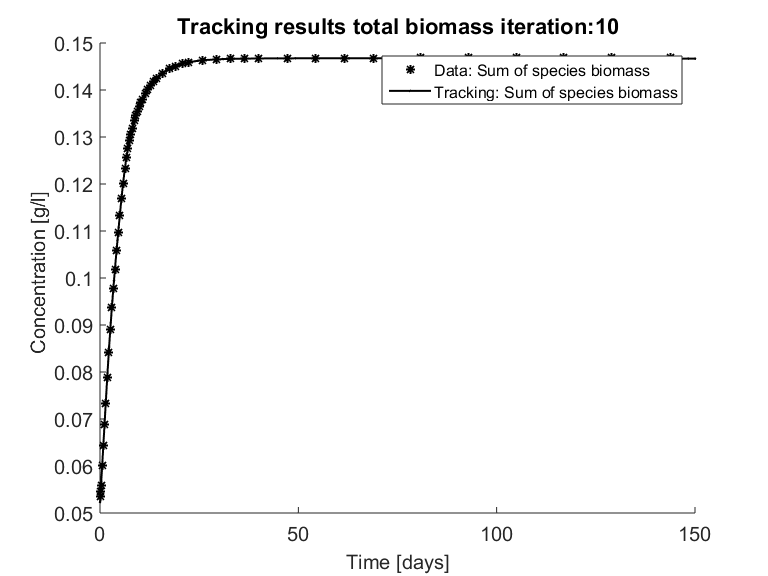
\includegraphics[width=0.5\textwidth]{Synthetic_data//lambda_=_e-1//191210_no_noise_Biomass_iter_10}
%	\caption{Total biomass. Dotted line: simulated data. Continuous line: the tracking procedure results.}
%	\label{Total Biomass no noise e1}
%\end{figure}
%\begin{figure}[h]
%	\centering
%	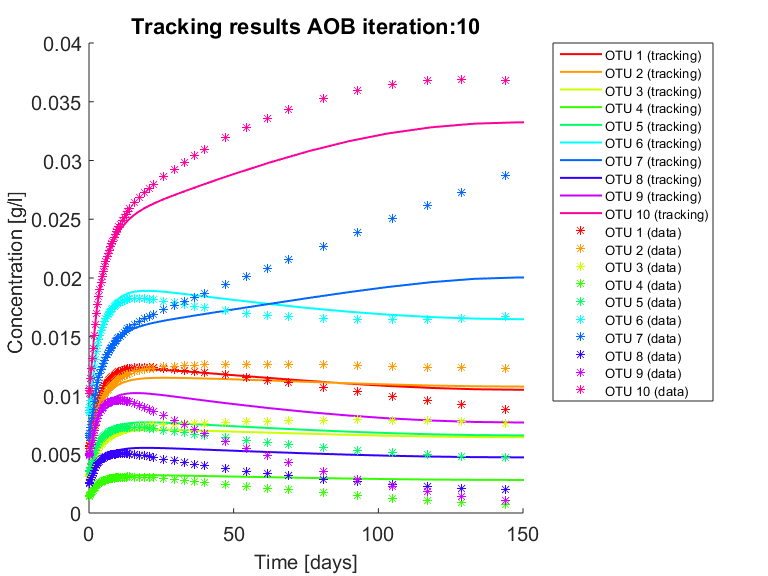
\includegraphics[width=0.5\textwidth]{Synthetic_data//lambda_=_e-1//191210_no_noise_AOB_iter_10_plot_1}
%	\caption{AOB biomass. Dotted line: simulated data. Continuous line: the tracking procedure results.}
%	\label{AOB no noise e1}
%\end{figure}
%\begin{figure}[h]
%	\centering
%	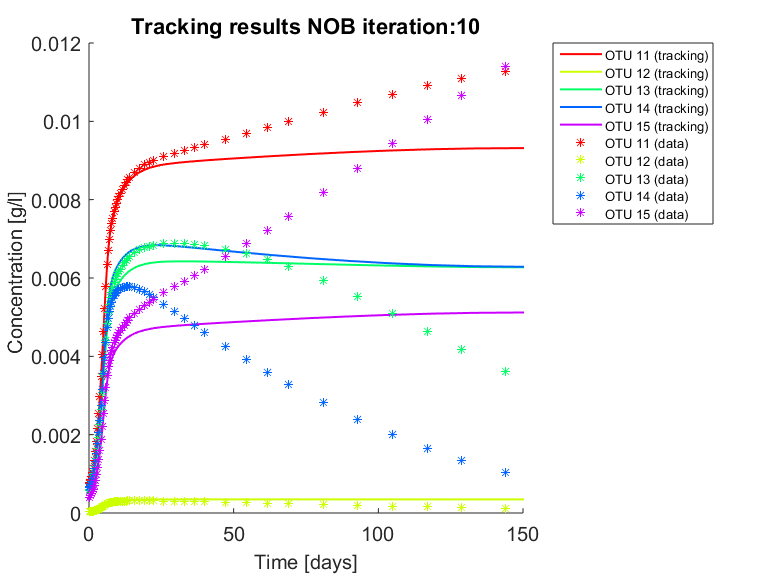
\includegraphics[width=0.5\textwidth]{Synthetic_data//lambda_=_e-1//191210_no_noise_NOB_iter_10_plot_1}
%	\caption{NOB biomass. Dotted line: simulated data. Continuous line: the tracking procedure results.}
%	\label{NOB no noise e1}
%\end{figure}
%\begin{figure}[h]
%	\centering
%	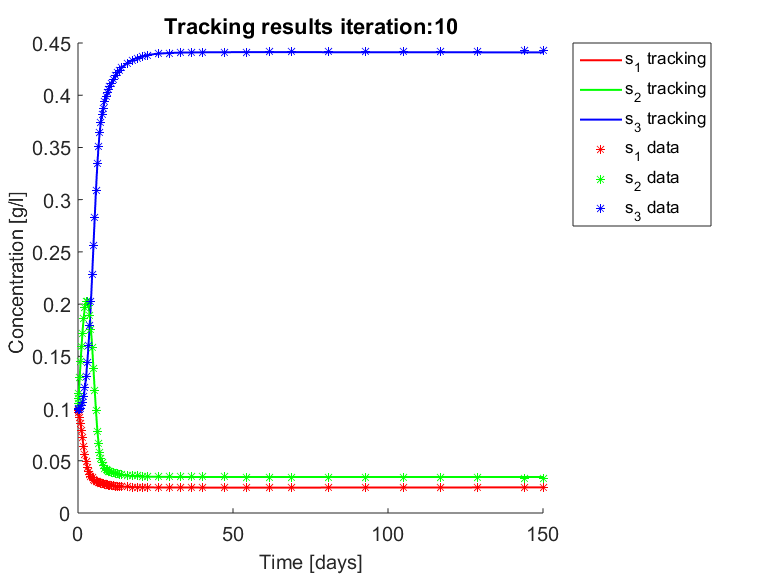
\includegraphics[width=0.5\textwidth]{Synthetic_data//lambda_=_e-1//191210_no_noise_metabolites_iter_10}
%	\caption{Metabolites. Dotted line: simulated data. Continuous line: the tracking procedure results.}
%	\label{Metabolites no noise e1}
%\end{figure}
%
%\begin{figure}[h]
%	\centering
%	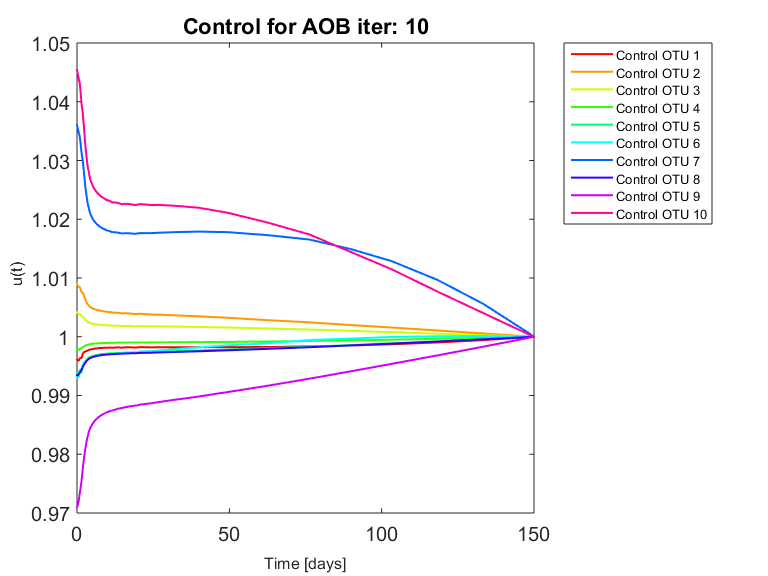
\includegraphics[width=0.5\textwidth]{Synthetic_data//lambda_=_e-1//191210_no_noise_Control_AOB_iter_10_plot_1}
%	\caption{Control for the AOB population.}
%	\label{Control AOB no noise e1}
%\end{figure}
%
%\begin{figure}[h]
%	\centering
%	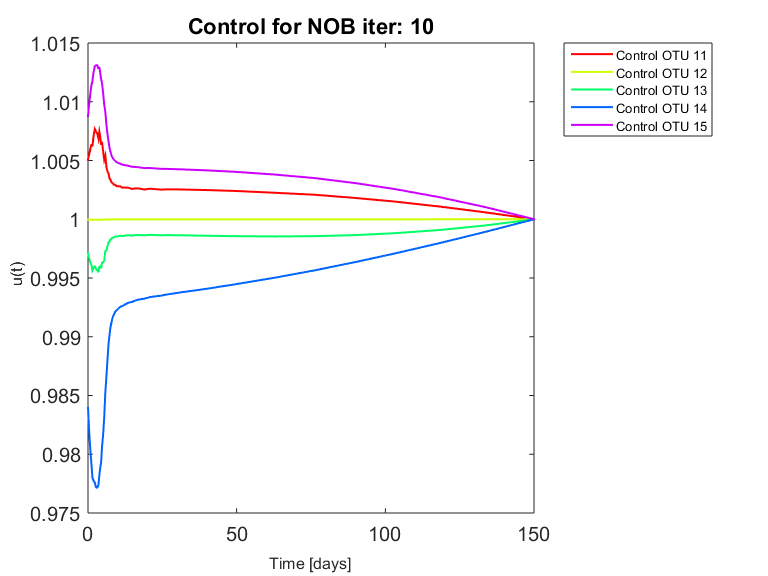
\includegraphics[width=0.5\textwidth]{Synthetic_data//lambda_=_e-1//191210_no_noise_Control_NOB_iter_10_plot_1}
%	\caption{Control for the NOB population.}
%	\label{Control NOB no noise e1}
%\end{figure}
%\clearpage
%\textbf{$\lambda = 10^{-2}$}
%\begin{figure}[h]
%	\centering
%	\includegraphics[width=0.5\textwidth]{Synthetic_data//lambda_=_e-2//191210_no_noise_2_Biomass_iter_10}
%	\caption{Total biomass. Dotted line: simulated data. Continuous line: the tracking procedure results.}
%	\label{Total Biomass no noise e2}
%\end{figure}
%\begin{figure}[h]
%	\centering
%	\includegraphics[width=0.5\textwidth]{Synthetic_data//lambda_=_e-2//191210_no_noise_2_Control_AOB_iter_10_plot_1}
%	\caption{AOB biomass. Dotted line: simulated data. Continuous line: the tracking procedure results.}
%	\label{AOB no noise e2}
%\end{figure}
%\begin{figure}[h]
%	\centering
%	\includegraphics[width=0.5\textwidth]{Synthetic_data//lambda_=_e-2//191210_no_noise_2_Control_NOB_iter_10_plot_1}
%	\caption{NOB biomass. Dotted line: simulated data. Continuous line: the tracking procedure results.}
%	\label{NOB no noise e2}
%\end{figure}
%\begin{figure}[h]
%	\centering
%	\includegraphics[width=0.5\textwidth]{Synthetic_data//lambda_=_e-2//191210_no_noise_2_metabolites_iter_10}
%	\caption{Metabolites. Dotted line: simulated data. Continuous line: the tracking procedure results.}
%	\label{Metabolites no noise e2}
%\end{figure}
%
%\begin{figure}[h]
%	\centering
%	\includegraphics[width=0.5\textwidth]{Synthetic_data//lambda_=_e-2//191210_no_noise_2_AOB_iter_10_plot_1}
%	\caption{Control for the AOB population.}
%	\label{Control AOB no noise e2}
%\end{figure}
%
%\begin{figure}[h]
%	\centering
%	\includegraphics[width=0.5\textwidth]{Synthetic_data//lambda_=_e-2//191210_no_noise_2_NOB_iter_10_plot_1}
%	\caption{Control for the NOB population.}
%	\label{Control NOB no noise e2}
%\end{figure}
%
%\clearpage

\section{References}
\bibliographystyle{elsarticle-num}
\bibliography{mybibfile}
\end{document}